% THIS IS AN EXAMPLE DOCUMENT FOR VLDB 2012
% based on ACM SIGPROC-SP.TEX VERSION 2.7
% Modified by  Gerald Weber <gerald@cs.auckland.ac.nz>
% Removed the requirement to include *bbl file in here. (AhmetSacan, Sep2012)
% Fixed the equation on page 3 to prevent line overflow. (AhmetSacan, Sep2012)
\listfiles
%\documentclass{sig-alternate}
\documentclass[conference]{IEEEtran}
\usepackage{graphicx}
\usepackage{amsmath}
\usepackage{color}
\usepackage{balance}  % for  \balance command ON LAST PAGE  (only there!)
\usepackage{times}
\usepackage{url}
\usepackage{algorithm}
\usepackage[noend]{algorithmic}
\usepackage{subfigure}
\usepackage{xspace}
\usepackage[noend]{algorithmic}
\usepackage{enumerate}
\usepackage{multirow}
\usepackage{epstopdf}
\usepackage{cleveref}
\usepackage{soul}
%\usepackage[font={small,it}]{caption}

\newcommand{\squishlist}{
   \begin{list}{$\bullet$}
    {
      \setlength{\itemsep}{0pt}
      \setlength{\parsep}{3pt}
      \setlength{\topsep}{3pt}
      \setlength{\partopsep}{0pt}
      \setlength{\leftmargin}{1.5em}
      \setlength{\labelwidth}{1em}
      \setlength{\labelsep}{0.5em} } }

\newcommand{\squishend}{
    \end{list}  }

\renewcommand*\ttdefault{cmvtt}

%\makeatletter
%\def\@copyrightspace{\relax}
%\makeatother


\newcommand{\argmax}{\operatornamewithlimits{arg\ max}}

\newcommand{\eat}[1]{}
\newcommand{\todo}[1]{\textcolor{red}{{TODO: #1}}}
\newcommand{\add}[1]{\textcolor{red}{{ADD: #1}}}
\newcommand{\note}[1]{\textcolor{blue}{{#1}}}
\newcommand{\agp}[1]{\textcolor{blue}{{Aditya: #1}}}
\newcommand{\stitle}[1]{\vspace{0.5em}\noindent\textbf{#1}}


\newtheorem{definition}{Definition}
\newtheorem{example}{Example}
\newtheorem{theorem}{Theorem}
\newtheorem{lemma}{Lemma}
\newtheorem{corollary}{Corollary}
\newtheorem{problem}{Problem}
\newtheorem{reduction}{Reduction}
\newcommand{\domain}{\mathcal{D}}
\newcommand{\attributes}{\mathcal{A}_D}
\newcommand{\hierarchy}{\mathcal{H}_D}
\newcommand{\attrhierarchy}{\mathcal{H}_A}
\newcommand{\workers}{\mathcal{W}}
\newcommand{\uentities}{\mathcal{E}}
\newcommand{\queryvector}{{\bf Q_S}}

\newif\ifpaper
\papertrue % comment out to create technical report

\newif\iftr
%\trtrue % uncomment to create technical report



\begin{document}

% ****************** TITLE ****************************************

%\title{CrowdGather: Entity Extraction over Structured Domains}
\title{CRUX: Crowdsourced Data Extraction from the Long Tail}
%\numberofauthors{3} 
%
%\author{
%	\alignauthor Theodoros Rekatsinas\\
%            \affaddr{University of Maryland, College Park} 
%                \email{thodrek@cs.umd.edu}
%            \alignauthor Amol Deshpande\\
%            \affaddr{University of Maryland, College Park} 
%                \email{amol@cs.umd.edu}
%            \alignauthor Aditya Parameswaran \\
%            \affaddr{University of Illinois, Urbana-Champaign} 
%                \email{adityagp@illinois.edu}
%}

\author{\IEEEauthorblockN{Theodoros Rekatsinas}
\IEEEauthorblockA{Stanford University\\
Email: thodrek@cs.stanford.edu}
\and
\IEEEauthorblockN{Amol Deshpande}
\IEEEauthorblockA{University of Maryland, College Park\\
Email: amol@cs.umd.edu}
\and
\IEEEauthorblockN{Aditya Parameswaran}
\IEEEauthorblockA{University of Illinois, Urbana-Champaign\\
Email: adityagp@illinois.edu}}

\maketitle

\begin{abstract}
Extracting and collecting information about real-world entities, such as people, organizations, and real-world events, in structured data repositories has enhanced our ability to interpret and understand content and offer personalized services. However, existing repositories suffer from a lack of fine-grained {\em long tail} data, i.e., the not-so-popular entities. In this paper, we examine how crowdsourcing techniques can be leveraged for entity extraction, thereby dramatically increasing coverage. We leverage two novel insights: {\em exploiting the structure of the domain of interest}, and {\em using exclude list to limit the repeated extractions}. We apply these insights in developing CRUX, a CRowdsoUrced data eXtraction framework that optimizes crowdsourced entity extraction by dynamically adapting the queries issued against the crowd to minimize the number of duplicate extractions, and thereby the wasted cost. We develop new statistical tools to reason about the gain, i.e., the number of new distinct extracted entities, of issuing {\em further queries} under the presence of little to no information; this allows us to effectively prune futile queries. We also introduce algorithms to discover adaptive querying strategies that maximize the number of distinct extracted entities under budget constraints. We evaluate our techniques on both synthetic and real-world datasets, demonstrating an improvement of up to 300\% over competing approaches for the same budget.
\end{abstract}

%!TEX root = ../crowd_hierarchies_kdd.tex

% THIS IS AN EXAMPLE DOCUMENT FOR VLDB 2012
% based on ACM SIGPROC-SP.TEX VERSION 2.7
% Modified by  Gerald Weber <gerald@cs.auckland.ac.nz>
% Removed the requirement to include *bbl file in here. (AhmetSacan, Sep2012)
% Fixed the equation on page 3 to prevent line overflow. (AhmetSacan, Sep2012)


\section{Introduction}
\label{sec:intro}

Structured data repositories, such as knowledge bases, taxono\-mies, and hierarchies, have recently been used to power end-user applications of many types, including keyword search engines, question answering systems, event detection and prediction algorithms, as well as recommender systems. For instance, a number of companies, including Google~\cite{singhal2012introducing}, Microsoft~\cite{cheng2010fuzzy}, Walmart~\cite{Deshpande:2013:BMU:2463676.2465297}, Yahoo~\cite{woo}, and Amazon~\cite{amazon-product}, all leverage structured data repositories for organizing and serving information for various applications. However, most automated mechanisms to populate these repositories end up focusing on {\em head data} --- data about popular entities, facts, and attributes --- leaving behind a considerable volume of fine-grained data belonging to the {\em long tail}. Thus, to obtain even more benefits from these repositories, it is essential to augment these repositories with long tail data, and keep them up-to-date. 

In the recent past, {\em crowdsourcing} has proven effective to gather structured data on demand~\cite{franklin:2011,deco, trushkowsky:2013, amsterdamer:2014, park:2014, kondredi:2014}. While automated mechanisms miss out on the {\em long-tail} data, crowdsourcing entity extraction has been shown to be capable of extracting data from the long-tail~\cite{trushkowsky:2013}. Prior work on this problem focuses on asking the same extraction query repeatedly to workers and studies the problem of determining when to stop the extraction process~\cite{trushkowsky:2013}. For example, given the task of collecting all modern philosophers, current techniques focus on asking workers to ``list one modern philosopher'' repeatedly until a certain desired degree of completeness is achieved.

However, while the previous work demonstrated that it is indeed possible to use crowds to extract entities, asking only one query to workers until completion means that the scheme will lead to the same entities---i.e., the popular ones---being repeatedly extracted by workers, while the not-so-popular ones will either never be extracted or only be extracted after a very long time. For example, the famous philosopher Bertrand Russell may be provided significantly more times than the less popular Greek-French philosopher Cornelios Castoriadis. This phenomenon, i.e., the skewed popularity of entities, can lead to increased duplicate extractions, rendering existing crowdsourced entity extraction techniques {\em impractical} for large-scale applications. 
\begin{table}[h]
\vspace{-10pt}\center
\caption{Extracting people from the news. Percentage of people reported by at least two different workers for each (occupation, news portal) combination. We collected a total of 150 entities for each combination.}
\label{tab:duplicates}
\begin{tabular}{|c|c|c|c|c|}
\hline
News Portal & {\bf Actors/Singer}s & {\bf Athletes} & \textbf{Politicians}\\ \hline
{\bf Wash. Post} & 0.47 & 0.55 & 0.56 \\
{\bf NY Times} & 0.41& 0.65 & 0.53 \\
{\bf Huff. Post} & 0.45 & 0.63 & 0.60 \\
{\bf USA Today} & 0.54 & 0.45 & 0.57 \\
{\bf WSJ} & 0.42 & 0.77 & 0.57 \\
\hline
\end{tabular}
\end{table}

\vspace{2pt}\noindent\textbf{The impact of duplicates.} To understand the impact of duplicate extractions, i.e., entities provided by multiple workers, we conducted a real entity extraction experiment using Amazon's Mechanical Turk (AMT)~\cite{mturk}. We focused on {\em extracting people from the news} and asked workers to list people of different occupations mentioned in five major online US news portals. More specifically, we asked workers to provide us with ``Actors/Singers'', ``Athletes'', and ``Politicians'' listed in ``New York Times'', ``Huffington Post'', ``Washington Post'', ``USA  Today'' and ``The Wall Street Journal''. For each (occupation, news portal) combination, e.g., ``Athletes mentioned in NY Times'', we asked 30 distinct workers to provide us with five entities leading to 150 extractions per combination. . 

\Cref{tab:duplicates} shows the percentage of entities that were provided by at least two different workers for different (occupation, news portal) combinations. As shown, on average, more than half of extracted entities we reported by at least two workers, while there are cases where the percentage of duplicated entities {\bf reaches 77\%}. This means that 77\% of the cost (in compensating workers for their answers) is simply wasted. 

Finally, we see that the percentage of duplicated entities varies significantly for different (occupation, news portal combinations). This leads to the natural question of {\bf which are the right crowd extraction queries that will maximize the total number of extracted entities?}. To address this question, we develop a framework for minimizing the number of duplicate extractions and focusing  extraction efforts (e.g., monetary cost) on long-tail entities.  

\vspace{2pt}\noindent\textbf{Our approach.} We introduce CRUX, a novel algorithmic framework for making {\em  crowdsourced entity extraction practical}. Unlike previous work, CRUX focuses on the problem of {\em budgeted crowdsourced entity extraction}, where we are given a budget and we want to maximize the number of retrieved entities; we believe this is a more practical goal, instead of the goal of retrieving all entities.  Effectively our goal is to minimize the total cost spent on duplicate extractions and maximize the total number of extracted entities. 

To do so, we focus on entity extraction over {\em structured domains}, i.e., domains that can be fully described by a collection of attributes, each potentially exhibiting hierarchical structure, and demonstrate how exploiting the domain's structure can help us achieve the aforementioned goal. For example, in our people extraction case, we could have one attribute about the occupation, one about the nationality, and one about the news portal. We can then leverage this entity domain to use a much richer space of queries asked to human workers, considering all combinations of values for each of these attributes, e.g., ``list a Cuban athlete mentioned in New York Times''. In this manner, we can leverage these specific, targeted queries to extract not-so popular entities with attribute values set to specific ones, e.g., in this case, nationality is ``Cuban'', occupation is ``athlete'', and news portal is ``New York Times''. 

In fact, most large-scale real-world applications that collect and organize information extracted by the crowd focus on structured domains. For example, we consider Eventbrite~(\url{www.eventbrite.com}), an online event aggregator, that relies on crowdsourcing to compile a directory of events, such as political rallies, concerts, etc. Events are fully described by their location, type, date and category. We point out that often the structure of domains in practical applications is already known by design and in many cases is also recorded in existing taxonomies or knowledge bases. Despite the above, existing work on crowdsourced entity extraction does not provide techniques to find the most profitable queries.

Using a richer space of crowd queries, allows us to avoid issuing the same query repeatedly. More precisely, if we view the structured data domain as a \emph{partially ordered set} (poset), then each query can be mapped to a node in the graph describing its topology. This allows for more targeted queries, e.g., ``list a Greek modern philosopher'', and enables us to explore a larger space of entities effectively by focusing on diverse and potentially disjoint groups of entities. Moreover, we extend typical crowd queries to also include an {\em exclude list}, e.g., ``list a modern philosopher that is not Bertrand Russell''. Both aforementioned approaches allow us to effectively reduce the number of duplicate extractions and enable us to extract more entities from the underlying domain (see \Cref{sec:exps}).

The ability to ask richer queries comes with a host of new challenges. First, we need to address the fundamental question: {\em Which is the most profitable query to issue next?}. For this, we propose a collection of  statistical techniques for estimating the {\em gain} of further queries, i.e., the number of new distinct entities extracted, for any node in the poset. Our techniques make use of the extracted entities by previously issued queries to derive accurate estimates for new queries corresponding to the nodes of the poset.  

However, the input poset is of exponential size with respect to the number of attributes describing the domain. This, leads to additional challenges in deciding which queries to issue: (a)~{\em Sparsity:} Many of the nodes in the poset are likely to be empty, i.e., the queries corresponding to those nodes are likely to not have any answers; avoiding asking queries corresponding to these nodes is essential to keep monetary cost low. (b)~{\em Limited information:} The larger the poset the fewer the observed entities corresponding to lower level nodes in the poset, thus, we only have limited information when estimating the gain of further queries at these nodes.  (c)~{\em Interrelationships:} Many of the nodes in the poset are ``coupled'' with one another; for example, the results from a few queries corresponding to ``list a political philosopher'' can inform whether issuing queries corresponding to ``list a German political philosopher'' is useful or not. 

In summary, our main contributions are as follows:
\squishlist
\item We formalize the notion of {\em generalized queries} that ask workers to provide us with entities from a domain $D$ and can also include an {\em exclude list}. In general such queries are of the type ``List $k$ entities with attributes $\bar{X}$ that belong in domain $D$ and are not in $\{A, B, ...\}$''.  We also provide a collection of statistical techniques to estimate the gain, i.e., the number of newly extracted distinct entities, for generalized queries. 
\item We develop a new technique to estimate the gain of generalized entity extraction queries under the presence of little information, i.e., only when a small portion of the underlying entity population has been observed. We empirically demonstrate its effectiveness when extracting entities from sparse domains.
\item We propose a novel algorithmic framework that exploits the structure of the entity domain to maximize the number of extracted entities under given budget constraints by targeting tail entities. In particular, we view the problem of entity extraction as a {\em multi-round adaptive optimization problem}. At  each round we exploit the available information about entities obtained by previous queries to adaptively select the next crowd query that will maximize the {\em cost-gain} trade-off at each round. 
\item Finally, we evaluate the effectiveness of our techniques on both real-world and synthetic data, and demonstrate that can extract 4X more entities over competing state-of-the-art techniques for the same budget.
\squishend

%Our main contributions are as follows:
%
%\squishlist
%\item We formalize the notion of an exclude list for crowdsourced entity extraction queries and show how previously proposed gain estimators can be extended to handle such queries.
%\item We develop a new technique to estimate the gain of generalized entity extraction queries under the presence of little information, i.e., only when a small portion of the underlying entity population has been observed. We empirically demonstrate its effectiveness when extracting entities from sparse domains.
%\item We introduce an adaptive optimization algorithm that takes as input the gain estimates for different types of queries and identifies querying policies that maximize the total number of retrieved entities under given budget constraints. 
%\item Finally, we show that our techniques can effectively solve the problem of budgeted crowd entity extraction for large data domains on both real-world and synthetic data.
%\squishend

%Previously proposed techniques~\cite{trushkowsky:2013} do not directly apply to the scenario where we are traversing a poset corresponding to this structured data domain, and new techniques are needed. The main limitation of the aforementioned techniques is that they focus on estimating the completeness of a specific fixed query and are agnostic to cost. As a consequence they do not address the problem of deciding which additional queries are \emph{worth} issuing.  To mitigate these shortcomings, one needs to tune the queries that are asked. However, deciding which queries to ask among a large number of possible queries (exponential in the number of attributes describing the input domain) and when and how many times to ask each query, are both critical challenges that need to be addressed. Furthermore, unlike previous work, we focus on the budgeted case, where we are given a budget and we want to maximize the number of retrieved entities; we believe this is a more practical goal, instead of the goal of retrieving all entities.  


%
%
%\iftr
%Our crowdsourced entity extraction techniques can be useful for a variety of entity extraction applications that are naturally coupled to a structured domain, including:
%\squishlist
%\item A newspaper that wants to collect a list of today's events to be displayed on the events page every day. 
%In this case, the structured data domain could include event type (e.g., music concerts vs.~political rallies) or location, among other attributes.
%\item A stock trading firm wants to collect a list of stocks that have been mentioned by popular press on the previous day. In this case, the structured data domain could include stock type, popular press article type, or whether the mention was positive or negative, among other attributes. 
%\item A real estate expert wants to curate a list of houses available for viewing today. The structured data domain in this case could include the price range, the number of floors, etc.
%\item A university wants to find all the faculty candidates on the job market. The structured data domain in this scenario includes the university of the applicant, specialization, and whether they are Ph.D./Postdoc.
%\item The PC chair of a new conference wants to find potential reviewers. The domain describing each of the candidates can be characterized by the university or company of the reviewer, expertise, qualifications, and so on. 
%\squishend
%\fi
%
%\subsection{Challenges in Structured Domains}
%\label{sec:challenges}
%To exemplify the aforementioned challenges we review a large-scale real-world scenario where crowdsourcing is used to extract entities. We consider Eventbrite~(\url{www.eventbrite.com}), an online event aggregator, that relies on crowdsourcing to compile a directory of events with detailed information about the location, type, date and category of each event. \iftr Typically, event aggregators are interested in collecting information about diverse events spanning from conferences and music festivals to political rallies across different location, i.e., countries or cities. In particular, \fi Eventbrite collects information about events across different countries in the world. Each country is split into cities and areas across the country. Moreover, events are organized according to their type and topic. The attributes and their corresponding structure are known in advance and are given by the design of the application. \iftr We collected a dataset from Eventbrite spanning over 63 countries that are divided into 1,709 subareas (e.g., states) and 10,739 cities, containing events of 19 different types, such as rallies, tournaments, conferences, conventions, etc. and a time period of 31 days spanning over the months of October and November. \fi
%
%Two of the three dimensions, i.e., location and time, describing the domain of collected events  are hierarchically structured. The poset characterizing the domain can be fully specified if we consider the cross product across the possible values for location, event type and time. For each of the location, time, type dimensions we also consider a special {\em wildcard} value. Taking the cross-product across the possible values of these dimensions results in poset with a total of 8,508,160 nodes containing 57,805 distinct events overall. We point out that the events associated with a node in the poset overlap with the events corresponding to its descendants. First, we demonstrate how the sparsity challenge applies to Eventbrite.
%\begin{example}
%We plot the number of events for each node in the poset describing the Eventbrite domain. Out of 8,508,160 nodes only 175,068 nodes are associated with events while the remaining have zero events. \Cref{fig:eventbritepop} shows the number of events per node (y-axis is in log-scale). Most of the populated nodes have less than 100 events. Additionally, the most populated nodes of the domain correspond to nodes at the higher levels of the poset. When extracting events from such a sparse domain one needs to carefully decide on the crowdsourced queries to be issued especially if operating under a monetary budget.
%\end{example}
%\iftr
%\begin{figure}
%	\begin{center}
%	\includegraphics[clip,scale=0.5]{figs/eventbritepop.eps}
%	\vspace{-10pt}
%	\caption{The population of different nodes in the Eventbrite domain.}
%	\label{fig:eventbritepop}
%	\vspace{-10pt}
%	\end{center}
%\end{figure}
%\fi
%
%\ifpaper
%\begin{figure}[h]
%	\centering
%	\vspace{-10pt}
%	\subfigure{\includegraphics[clip,scale=0.32]{figs/eventbritepop.eps}\label{fig:eventbritepop}}
%	\hspace{-10pt}
%	\subfigure{\includegraphics[clip,scale=0.32]{figs/overlaps.eps}\label{fig:eventbriteover}}
%	\vspace{-10pt}
%	\caption{(a) The population of different nodes and (b) pairwise overlaps for the 10 most populous nodes in the Eventbrite domain.}
%	\vspace{-10pt}
%\end{figure}
%\fi
%
%As mentioned before, a critical challenge in such large domains is deciding on the queries to ask. However, the hierarchical structure of the data domain presents us with an opportunity. One approach would be to perform a top-down traversal of the poset and issue queries at the different nodes. Nevertheless, this gives rise to a series of challenges: (i) how can one decide on the number of queries to be asked at each node, (ii) when should one progress to deeper levels of the poset and (iii) which subareas should be explored. We elaborate on these in \Cref{sec:prelims}. Next, we focus on the second challenge, i.e., the interdependencies across poset nodes. 
%\begin{example}
%We consider again the Eventbrite dataset and plot the pairwise overlaps of the ten most populous nodes in the domain. \Cref{fig:eventbriteover} shows the Jaccard index for the corresponding node pairs. As shown the event populations corresponding to these nodes overlap significantly. It is easy to see that when issuing queries at a certain domain node, we not only obtain events corresponding to this node but to other nodes in the domain as well.
%\end{example}
%A critical issue that stems from the overlaps across nodes is being able to decide how many answers to expect when issuing an additional query at a node whose underlying population overlaps with nodes associated with previous queries. In \Cref{sec:prelims}, we elaborate more on the dependencies across nodes of the poset.
%\iftr
%\begin{figure}
%	\begin{center}
%	\includegraphics[clip,scale=0.5]{figs/overlaps.eps}
%	\vspace{-10pt}
%	\caption{Pairwise overlaps for the 10 most populous nodes.}
%	\label{fig:eventbriteover}
%	\vspace{-10pt}
%	\end{center}
%\end{figure}
%\fi
%\subsection{Contributions}
%\label{sec:contributions}
%Motivated by the examples above, we study the problem of crowdsourced entity extraction in the presence of long tail data. To effectively extract entities from the long tail we focus on {\em structured domains}. More precisely, we focus on domains described by a collection of attributes, each following a known {\em hierarchical structure}, i.e., we assume that for each attribute the corresponding hierarchy is known. Such hierarchies are usually dictated by the design of applications. \iftr Moreover, as controlling the overall extraction cost in large-scale applications is crucial we focus on {\em budgeted crowd entity extraction}. \fi
%
%We propose a novel algorithmic framework that exploits the structure of the domain to maximize the number of extracted entities under given budget constraints by targeting tail entities. In particular, we view the problem of entity extraction as a {\em multi-round adaptive optimization problem}. At  each round we exploit the information on extracted entities obtained by previous queries to adaptively select the crowd query that will maximize the {\em cost-gain} trade-off at each round. The gain of a query is defined as the {\em number of new unique entities extracted}. 
%
%We consider {\em generalized queries} that ask workers to provide us with entities from a domain $D$ and can also include an {\em exclude list}. In general such queries are of the type ``Give me $k$ more entities with attributes $\bar{X}$ that belong in domain $D$ and are not in $\{A, B, ...\}$''. Extending techniques from the species estimation and building upon the multi-armed bandits literature, we introduce a new methodology for estimating the gain for such generalized queries and show how the hierarchical structure of the domain can be exploited to increase the number of extracted entities. Our main contributions are as follows:
%
%\squishlist
%\item We formalize the notion of an exclude list for crowdsourced entity extraction queries and show how previously proposed gain estimators can be extended to handle such queries.
%\item We develop a new technique to estimate the gain of generalized entity extraction queries under the presence of little information, i.e., only when a small portion of the underlying entity population has been observed. We empirically demonstrate its effectiveness when extracting entities from sparse domains.
%\item We introduce an adaptive optimization algorithm that takes as input the gain estimates for different types of queries and identifies querying policies that maximize the total number of retrieved entities under given budget constraints. 
%\item Finally, we show that our techniques can effectively solve the problem of budgeted crowd entity extraction for large data domains on both real-world and synthetic data.
%\squishend

%
%
%
%\noindent\textbf{Our approach.} In this paper, we focus on entity extraction over {\em structured domains}, i.e., domains that can be fully described by a collection of attributes, each potentially exhibiting hierarchical structure, and demonstrate how exploiting the domain's structure can help us achieve the aforementioned goal. 
%In fact, most practical  applications that focus on aggregating and organizing information extracted from the crowd exhibit some form of structure. 
%
%
%To do so, we focus on entity extraction over {\em structured domains}, i.e., domains that can be fully described by a collection of attributes, each potentially exhibiting hierarchical structure, and demonstrate how exploiting the domain's structure can help us achieve the aforementioned goal. We point out that often the structure of domains in practical applications is already known by design. For example, Eventbrite categorizes extracted events based on a location taxonomy, an event type and their date. 
%
%Naturally, we should exploit the {\em structure} of the entity extraction domain, here, the entity-type and news portal, to minimize the number of duplicate extractions.
%
%\noindent\textbf{Structured entity domains.}
%An additional limitation of existing crowdsourced entity extraction techniques is that they are agnostic to the inherent {\em structure} that large-scale entity domains exhibit. In most practical scenarios, the entity domain can be described by a collection of attributes. For instance, if we consider the previous example of extracting modern philosophers, it is easy to see that the underlying domain can be described by attributes such as the nationality of a philosopher, her school of thought and her era. In fact many real-world crowdsourcing applications rely on s
%
%Exploiting the structure of the domain allows one to issue a collection of queries with different predicates corresponding to various attribute combinations. The latter is indeed used in real-world crowdsourcing applications. 
%
%
%\begin{example}
%We considered the application of enumerating ``people in the news''. We asked workers to consider five major online US news portals, ``New York Times'', ``Huffington Post'', ``Washington Post'', ``USA  Today'' and ``The Wall Street Journal'', and report five distinct people per HIT. We issued 600 HITs for \$0.20 per HIT served by 143 unique workers. To ensure the accuracy of our results we asked workers to provide us with a link corresponding to the extraction. These links were manually verified.  In total, we extracted 1,245 unique people. \Cref{fig:amtPop} shows the number of distinct workers that reported each person. As shown, there are 12 people that were reported by at least 20 different workers but there is a long tail of 842 people that were reported by one worker and 182 people reported by two workers. 
%\end{example}
%
%To understand the impact of duplicate extractions we conducted the following experiment. We asked workers via Amazon's Mechanical Turk (AMT)~\cite{mturk} to list 
%
%The situation only becomes worse when entities follow a skewed, long tail {\em popularity distribution}, i.e., a small number of entities have significantly higher probability of appearing in worker answers while a large number of {\em rare} entities have minuscule probability of being extracted. Next, we consider two crowdsourced entity extraction applications to demonstrate the presence of long tail popularity distributions and exemplify how they can lead to increased numbers of duplicate extractions.
%
%\textcolor{red}{
%\begin{enumerate}
%\item There are many extraction domains that exhibit structure. Different from simple domains such as list all ice cream flavors. Example, online aggregation of events, extraction of named entities etc. Diversification important. 
%\item Show why. Example, extract humans from different news papers. We see that we have different duplicate rates for different predicate combinations. How can we reason about which predicates to include in our queries? Work on example.
%\end{enumerate}
%}
%
%\begin{figure*}
%	\centering
%	\subfigure[Event popularity in EventBrite.]{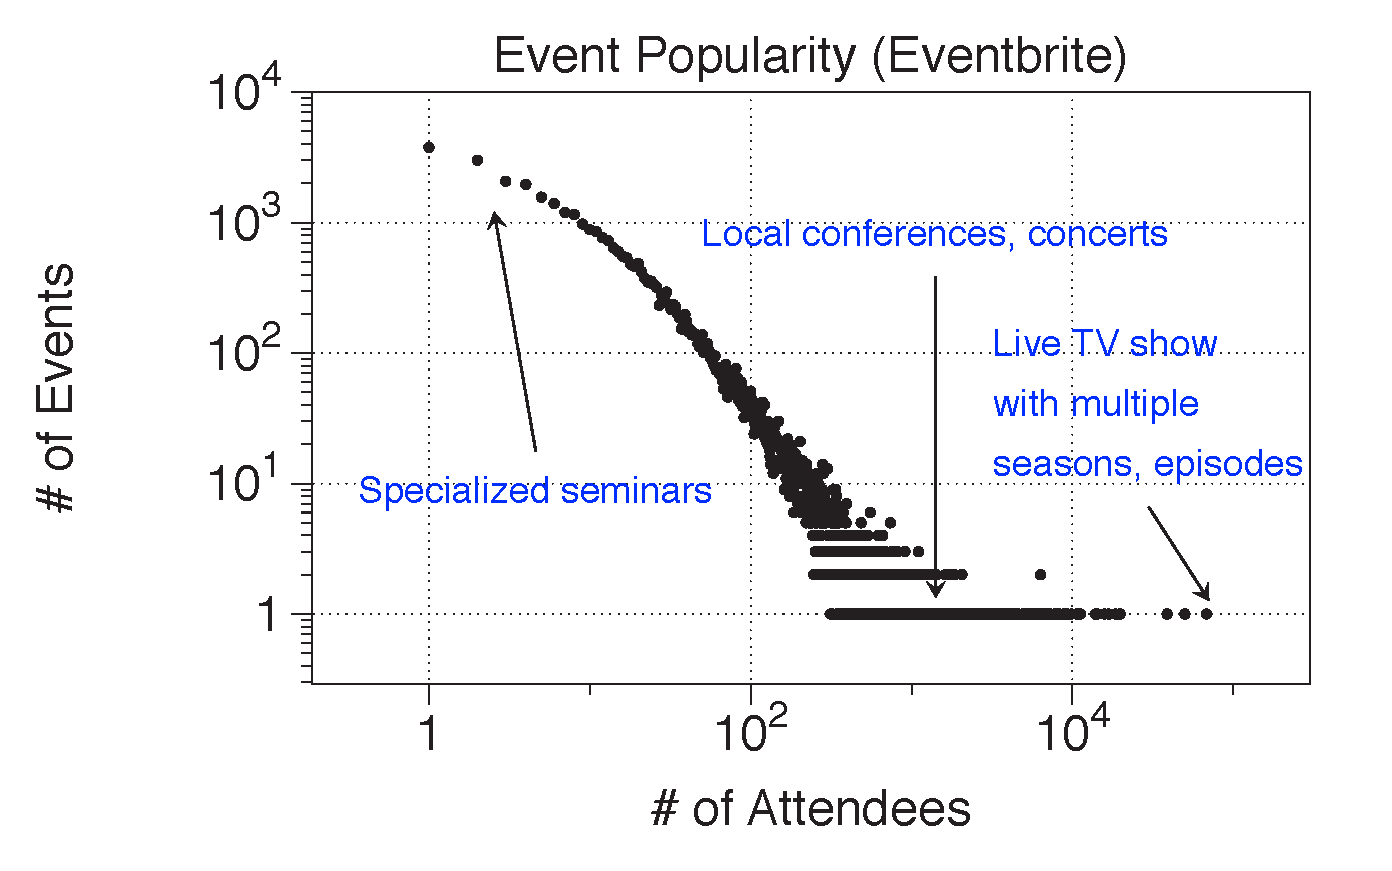
\includegraphics[clip,scale=0.35]{figs/eventPop.eps}\label{fig:eventPop}}
%	\subfigure[Entity popularity in crowdsourced people extraction.]{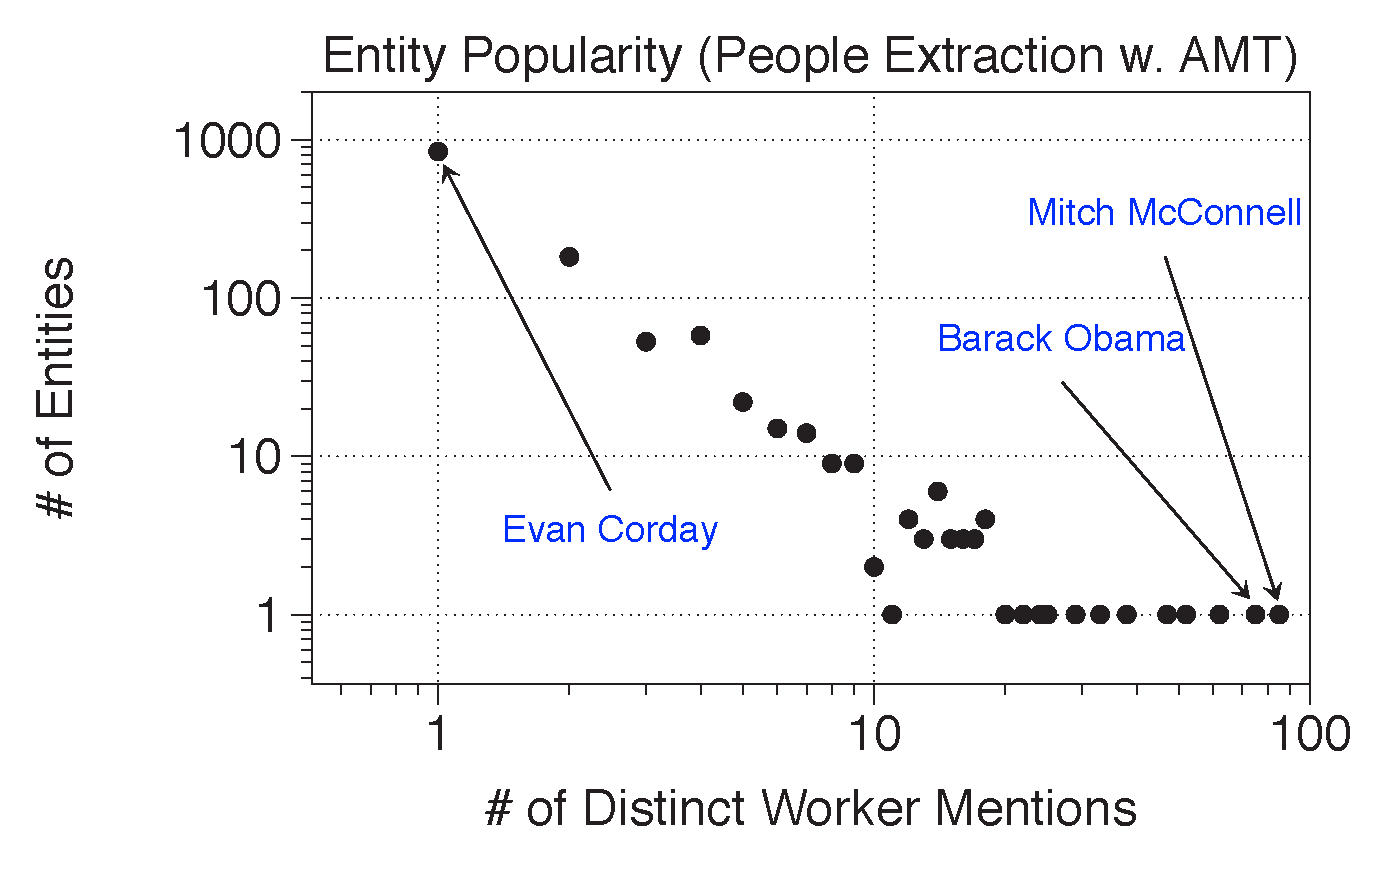
\includegraphics[clip,scale=0.35]{figs/amtPop.eps}\label{fig:amtPop}}
%	\caption{Entity popularity distributions exhibit long tails in real crowdsourced entity extraction applications.}
%\end{figure*}
%
%\begin{example}
%First, we consider Eventbrite~(\url{www.eventbrite.com}), an online event aggregator, that relies on crowdsourcing to compile a directory of events with detailed information about the location, type, date and category of each event. We collected a dataset via Eventbrite's API with events of 19 different categories from 63 different countries over a time period of 31 days. To measure the popularity of each event we use as a surrogate the number of attendees that registered for a specific event via Eventbrite.  In \Cref{fig:eventPop} we plot the number of registered attendees for different events grouping together events that had the same number of attendees. As shown, there is a large number of events with less than 100 attendees corresponding mostly to specialized seminars, and a small number of extremely popular events corresponding to concerts or live TV shows. 
%\end{example}
%
%\agp{not super clear how you plotted this}
%
%As we did not have immediate access to crowd workers for the aforementioned application, we also conducted a real crowdsourcing experiment via Amazon's Mechanical Turk (AMT)~\cite{mturk} that allowed us to precisely measure the popularity of extracted entities. 
%
%\begin{example}
%We asked workers to extract ``people in the news''. In particular, we asked them to consider five major online US news portals, ``New York Times'', ``Huffington Post'', ``Washington Post'', ``USA  Today'' and ``The Wall Street Journal'', and report five distinct people per HIT. We issued 600 HITs for \$0.20 per HIT served by 143 unique workers. To ensure the accuracy of our results we asked workers to provide us with a link corresponding to the extraction. These links were manually verified.  In total, we extracted 1,245 unique people. \Cref{fig:amtPop} shows the number of distinct workers that reported each person. As shown, there are 12 people that were reported by at least 20 different workers but there is a long tail of 842 people that were reported by one worker and 182 people reported by two workers. 
%\end{example}
%
%\agp{The examples are nice. Note that it's not clear what reporting means or
%what the workers are asked ---
%we need to stick to one of query, question, extract, report, etc.}
%
%\agp{CRUX, if we're using the acronym, needs to be introduced in the intro,
%not just in abstract.}
%
%\agp{Not super clear what the two graphs show -- i guess it's just that 
%we have a skewed probability distribution?
%can we also make the claim that: 
%there are actually just N entities:
%would it be possible to extract all entities using N or close to N crowd extractions, as opposed to using KN extractions, which is
%what we would have if we used repeated simple queries}
%
%\agp{got until here. }
%!TEX root = ../crowd_hierarchies_kdd.tex

\section{Preliminaries}
\label{sec:prelims}
In this section we provide the necessary definitions and background for formalizing the problem of crowdsourced entity extraction when considering structured domains. First, we define the notion of a structured domain, then describe the association between entities and the poset describing a structured domain. We continue by describing 
entity extraction queries and interfaces over structured domain, along with the response and cost model for these queries. Finally, we define the problem of {\em budgeted crowd entity extraction} over {\em structured domains} that seeks to maximize the number of extracted entities under budget constraints and present an overview of our proposed framework.


\subsection{Structured Data Domain}
\label{sec:data-domain}

Let $\domain$ be a data domain described by a set of discrete attributes $\attributes = \{A_1, A_2, \dots, A_d\}$. Let $dom(A_i)$ denote the domain of each attribute $A_i  \in \attributes$. We consider domains where each attribute $A_i$ can also be hierarchically organized. \iftr For example, consider the Eventbrite domain introduced in \Cref{sec:challenges}. The data domain $\domain$ corresponds to all events and the attributes describing the entities in $\domain$ are $\attributes = \{$``Event Type'', ``Location'', ``Date''$\}$. \Cref{fig:eventsdomain} shows the hierarchical organization of each attribute.

\begin{figure}[h]
	\begin{center}
	\includegraphics[clip,scale=0.33]{figs/eventsDomain.eps}
	\vspace{-10pt}
	\caption{The attributes describing the Eventbrite domain and the hierarchical structure of each attribute.}
	\label{fig:eventsdomain}
	\end{center}
	\vspace{-20pt}
\end{figure}
\fi
\ifpaper
For Eventbrite, introduced in \Cref{sec:intro}, the entities in the data domain $\domain$ correspond to events. The attributes describing the entities in $\domain$ are $\attributes = \{$``Event Type'', ``Location'', ``Date''$\}$, with ``Location'' and ``Date'' being hierarchically organized.
\fi
The domain $\domain$ can be viewed as a {\em poset}, i.e., a partially ordered set, corresponding to the cross-product of all available hierarchies\footnote{Note that $\domain$ is not a lattice since there is no unique infimum.}. Part of the poset corresponding to the previous example is shown in \Cref{fig:eventslattice}. We denote the poset for a domain $\domain$ as $\hierarchy$. As shown in \Cref{fig:eventslattice}, nodes in the poset me correspond to configurations where only a subset of the attributes in $\attributes$ are specified while others are allowed to take any value. For example the root of the poset $\{\}$ has no specified attributes allowing for queries of the form ``list an event''. Nodes at lower levels, such as $\{X1\}$ and $\{C1\}$, correspond to queries where the event type and location are specified respectively. 

\begin{figure}[h]
	\begin{center}
	\includegraphics[clip,scale=0.3]{figs/eventsExLattice.eps}
	\caption{Part of the poset defining the entity domain for Eventbrite.}
	\label{fig:eventslattice}
	\end{center}
\end{figure}

\subsection{Entities and Entity Extraction Queries}
\label{sec:queries}

\stitle{Entities.} Our goal is to extract entities that belong to the domain $\domain$. We assume that each entity $e$ can be uniquely associated with one of the leaf nodes in the hierarchy $\hierarchy$; that is, there is a unique combination of attribute values $A_1, \ldots, A_d$ characterizing each entity. For example, in Eventbrite, each entity (here, a local event) is of a specific type, takes place in a specific city, and on a specific day. Our techniques are also applicable when entities are underspecified, i.e., only a subset of the attributes in $\attributes$ are specified, but we focus on the former case for simplicity.

\stitle{Queries.} Next, we introduce the notion of {\em generalized extraction queries} that can be issued against crowd workers. We require that a query $q^v$ is associated with a node $v \in \hierarchy$; that is a query contains predicates that correspond to zero or more attribute in $\attributes$ and the predicates correspond to the value combination for $\attributes$ associated with $v$. For example, if we consider the poset shown in \Cref{fig:eventslattice} a query for node $\{X1\}$ has a predicate $EventType = X1$. Hence, workers are required to provide entities, here, events, that satisfy this predicate, i.e., they are of type $X1$.

Given a query $q^v$ associated with node $v \in \hierarchy$, we consider three different further configurations for  extracting entities from the crowd: The first configuration corresponds to {\em single entity queries} where workers are required to provide only ``one more'' entity matching the predicates of the query. Considering the Eventbrite example introduced in the previous section, an example of a single entity query would be asking a worker to provide ``a concert in New York'', where the predicates are $\mathsf{EventType = concert}$ and $\mathsf{State = New York}$. The second configuration corresponds to {\em queries of size k} where workers are asked to provide $k$ distinct entities for a query $q^v$. Finally, the last configuration corresponds to {\em exclude list queries}. Here,  workers are additionally provided with a list $E$ of $l$ entities that have already been extracted and are required to provide $k$ distinct entities that are not present in the exclude list. It is easy to see that the last configuration generalizes the previous two. Therefore, in the remainder of the paper, we will only consider queries using the third configuration. We refer to these queries as {\em generalized}. To describe a generalized query, we will use the notation $q^v(k,E)$ denoting a query of size $k$ accompanied with an exclude list $E$ of length $l$ and associated with node $v \in \hierarchy$. We will denote the configuration characterizing the query as $(k,l,v)$. 

\stitle{Query Response.} Given a query $q^v(k, E)$ issued at a node $v \in \hierarchy$, a human worker gives us $k$ distinct entities that belong to the domain $\domain$, match the query predicates and are not present in $E$. Furthermore, we consider a querying interface that asks human workers to not only list entities but to also provide,  for each entity, the values to the remaining attributes in $\attributes$ that are not specified in the predicates of $q$. For example, if our query is ``list one concert in Manhattan, New York'', with $k = 1, E = \emptyset$, the human worker gives us one concert in Manhattan, New York, but also gives us the day on which the concert will take place (here, the missing, unspecified attribute) and potentially the type of concert, i.e,. rock concert. If the query is ``a concert in the US'', with $k = 1, E = \emptyset$, the human worker gives us one concert in the US, but also gives the day on which the concert will take place, as well as the specific city. If less than $k$ entities are present in the underlying population, workers have the flexibility to report either an empty answer or a smaller number of entities (\Cref{sec:excludelist}).

While the reader may wonder if getting additional attribute values for entities is necessary, we note that this information allows us to assign an extracted entity to all nodes in $\hierarchy$ the entity belongs to; without this, it is difficult to effectively collect information about the underlying entity population associated with each node in the poset. Furthermore, we find that in most practical applications, it is useful to get the values of the missing attributes to organize and categorize the extracted entities better. Similar query interfaces that ask users to fully specify the attributes of entities have been proposed in recent literature~\cite{quinn:2014}. 

\ifpaper \stitle{Detecting Duplicate Entities.} Finally, answers are expected to be duplicated across workers, who may also provide an entity incorrectly. Resolving duplicates during extraction is crucial as they are used to estimate the completeness of extracted entities, and thus, reason about the gain of additional queries. In practice, standard entity resolution techniques~\cite{getoor:kdd13} using simple rules matching the attribute values of entities can be used to address this problem. Detecting duplicate extractions across worker answers is crucial to estimate the popularity distribution governing the extraction domain under consideration and estimate the gain of additional queries at different nodes of the poset $\hierarchy$. Nevertheless entity resolution is an orthogonal problem and not the focus of this paper. \fi

\iftr
Finally, answers are expected to be duplicated across workers, who may also specify or extract an entity incorrectly. Resolving duplicate entities during extraction is crucial as this information is later used to estimate characterize the completeness of extracted entities, and thus, reason about the gain of additional queries.  Extraction errors can be resolved by leveraging the presence of duplicate information and by applying de-duplication and entity resolution techniques. At a high-level one can use an entity resolution or string similarity (e.g., jaccard coefficient) algorithm to identify duplicate entities. Furthermore, the additional attributes for each entity, can be used to further ascertain similarity of entities. We refer the user to Getoor and Machanavajjhala~\cite{getoor:kdd13} for an overview of entity resolution techniques. Finally, standard truth discovery techniques can be used to identify the correct attribute values for entities. Nevertheless entity resolution and truth discovery are orthogonal problems and not the focus of this paper. In our experiments on real datasets, we found that there were no cases where humans introduced errors to the attribute values of extracted entities. Only minor errors (e.g., misspelled entity names) were detected and fixed manually. \fi

\stitle{Query Cost.} In a typical crowdsourcing marketplace, tasks have different costs based on their difficulty. Thus, crowdsourced queries of different difficulties should also exhibit different costs. We assume we are provided with a cost function $c(\cdot)$ that obeys the following properties:  (a) given a query with fixed size its cost should increase (or remain the same) as the size of its exclude list is increasing, (b) given a query with a fixed exclude list size its cost should increase (or remain the same) as the number of requested answer increases, and (c) given a query with fixed size and exclude list size its cost should increase (or remain the same) as the query contains more predicates, i.e., it corresponds to nodes $v$ at the lower-levels of $\hierarchy$. These are fixed upfront by the interface-designer based on the amount of work involved.

\subsection{Crowdsourced Entity Extraction}
\label{sec:extraction}
The basic version of {\em crowdsourced entity extraction}~\cite{trushkowsky:2013} seeks to extract entities that belong to $\domain$, by simply using repeated queries at the {\em root node}, with $k = 1, E = \emptyset$. When considering large entity domains, one may need to issue a series of entity extraction queries at multiple nodes in  $\hierarchy$ --- often overlapping with each other --- so that the entire domain is covered. Issuing queries at different nodes ensures that the coverage across the domain will be maximized. 

We let $\pi$ denote a {\em querying policy}, i.e., a series of $q^v(k,E)$ queries at different nodes $v \in \hierarchy$. A policy $\pi$ can select a query $q^v(k,E)$ multiple times. Let $C(\pi)$ denote the overall cost, in terms of monetary cost of a querying policy $\pi$. We define the gain of a querying policy $\pi$ to be the total number of unique entities, denoted by $\uentities(\pi)$ extracted when following policy $\pi$. Thus, there is a natural tradeoff between the gain (i.e., the number of extracted entities) and the cost of policies. 

Here, we require that the user will {\em only} provide a monetary budget $\tau_c$ imposing a constraint on the total cost of a selected querying policy, and optimize over all possible querying policies across different nodes of $\hierarchy$. The poset $\hierarchy$ and the possible query configurations $(k,l)$ for each node, i.e., the possible query sizes and exclude list sizes are given as input by the designer. Our goal is to identify the policy that maximizes the number of retrieved entities under the given budget constraint. More formally, we define the problem of budgeted crowd entity extraction as follows:

\begin{problem}[Budgeted Crowd Entity Extraction] \ \\
Let $\domain$ be a given entity domain characterized by a poset $\hierarchy$. For each node $v \in \hierarchy$ let $K^v$ and $L^v$ be the sets of allowed query sizes and exclude list sizes for query at node $v$ respectively. Also let $\tau_c$ a monetary budget on the total cost of issued queries. The Budgeted Crowd Entity Extraction problem seeks to find a querying policy $\pi^*$ using queries $q^v(k,E)$ with $k \in K^v$ and $|E| = l \in L^v$ over nodes $v \hierarchy$ that maximizes the number of unique entities extracted $\uentities(\pi^*)$ under the constraint $C(\pi^*) \leq \tau_c$.
\end{problem}
Notice, that the optimal policy not only specifies the nodes at which queries will be executed but also the size and exclude list of each query. The cost of a querying policy $\pi$ is defined as the total cost of all queries issued by following $\pi$. We have that $C(\pi) = \sum_{q \in \pi} c(q)$ where the cost of each query $q^v$ is defined according to a cost model specified by the user. 

\begin{theorem}
The problem of Budgeted Crowd Entity Extraction is NP-hard.
\end{theorem}
The proof is provide in \Cref{sec:prth1} in the Appendix and is based on a reduction from the unbounded knapsack problem. The latter is a variation of the original 0-1 knapsack problem that places no upper bound on the number of copies of each kind of item.

Finally, we note that computing the total cost of a policy $\pi$ is easy. However, the gain $\uentities(\pi)$ of a policy $\pi$ is unknown as we do not know in advance the entities corresponding to each node in $\hierarchy$, and hence, needs to be estimated, as we discuss in \Cref{sec:gainestimators}. 

\subsection{Underlying Query Response Model}
\label{sec:sampling}
To reason about the occurrence of entities as response to specific queries, we need an underlying query response model. Our query response model is based on the notion of {\em popularity}.
\ifpaper We assume that each underlying entity has a {\em unknown popularity value} with respect to crowd workers. Since workers are likely to return different answers based on how the query is phrased, this popularity can be different for different nodes in $\hierarchy$, and thus, query dependent. 
Given a query $q^v(1, \emptyset)$, asking for one entity from node $v$ without using an exclude list, the probability that we will get entity $e$ that satisfies the constraints specified by the predicates associated with node $v$ is nothing but the popularity value of $e$ divided by the popularity value of all entities $e'$ that also satisfy the same predicate constraints. As an example, if there are only two entities $e_1, e_2$ that satisfy the constraints specified by a given query $q_1$, with popularity values $3$ and $2$, then the probability that we get $e_1$ on issuing a query $q_1(1, \emptyset)$ is 3/5. If an exclude list $E$ is specified, then the probability that we will get an entity $e \notin E$ is the popularity value of $e$ divided by the popularity values of all entities $e' \notin E$ also satisfying the constraints specified by $q^v$. {\bf We do not assume that all workers follow the same popularity distribution}. Rather the overall popularity distribution can be seen as an average of the popularity distributions across all workers.

Since workers are asked to provide a limited number of entities as response to a query, each entity extraction query can be viewed as taking a random sample from an unknown population of entities. We refer to the distribution characterizing the popularities of entities in a population of entities as the {\em popularity distribution} of the population. Then, estimating the gain of a query $q^v(k,E)$ at a node $v \in \hierarchy$ is equivalent to estimating the number of new entities extracted by taking additional samples from the population of $v$ given all the retrieved entities (i.e., {\em running sample}) associated with node $v$. Due to the structure of the poset we may retrieve entities for a node when issuing queries at other nodes. We discuss this form of {\em indirect sampling} in \Cref{sec:gainestimators}. 
\fi
\iftr
\stitle{Popularities.} We assume that each underlying entity has a {\em fixed, unknown popularity value} with respect to crowd workers. Given a query $q(1, 0)$, asking for one entity and using an exclude list of size $0$, the probability that we will get entity $e$ that satisfies the constraints specified by $q$ is nothing but the popularity value of $e$ divided by the popularity value of all entities $e'$ that also satisfy the constraints in $q$. As an example, if there are only two entities $e_1, e_2$ that satisfy the constraints specified by a given query $q_1$, with popularity values $3$ and $2$,
then the probability that we get $e_1$ on issuing a query $q_1(1, 0)$ is 3/5. 
If an exclude list $S$ is specified, then the probability that we will get an entity $e \notin S$ is the popularity value of $e$ divided by the popularity values of all entities $e' \notin S$ also satisfying the constraints specified by $q$. Note that, we {\bf do not assume that all workers follow the same popularity distribution}. Rather the overall popularity distribution can be seen as an average of the popularity distributions across all workers.

Thus, since workers are asked to provide a limited number of entities as response to a query, each entity extraction query can be viewed as taking a random sample from an unknown population of entities. In the rest of the paper, we will refer to the distribution characterizing the popularities of entities in a population of entities as the {\em popularity distribution} of the population. We note that this is equivalent to the underlying assumption in the species estimation literature~\cite{chao:1992} (\Cref{sec:gainestimators}).

% We assume that the underlying entities exhibit different {\em popularity levels} with respect to crowd workers. These popularity levels can be formally defined using the notion of a probability distribution. In particular, the probability that an entity will appear as part of a query result depends on its {\em popularity} relative to the overall entity population. The popularity of an entity for a query $q$ is defined as the probability that this entity will appear in a query $q(1,0)$, i.e., a query asking for one entity from the population and using an exclude list of size zero. Since workers are asked to provide a limited number of entities as response to a query, each entity extraction query can be viewed as taking a random sample from an unknown population of entities. In the remainder of the paper, we will refer to the distribution characterizing the popularities of entities corresponding to a population as the {\em popularity distribution} of the population. 

Then, estimating the gain of a query $q(k,l)$ at a node $v \in \hierarchy$ is equivalent to estimating the number of new entities extracted by taking additional samples from the population of $v$ given all the retrieved entities by past samples associated with node $v$~\cite{trushkowsky:2013}. 

\stitle{Samples for a Node.} When extracting entities,  the retrieved entities for a node $v$ can correspond to two different kinds of samples: (i) those that were extracted by considering the {\bf entire population} corresponding to node $v$ (ii) and those that we obtained by sampling {\bf only a part of the population} corresponding to $v$. Samples for a node $v$ can be obtained either by querying node $v$ or by indirect information flowing to $v$ by queries at other nodes. We refer to the latter case as {\em dependencies across queries}. 
\begin{figure}[h]
	\begin{center}
	\vspace{-10pt}
	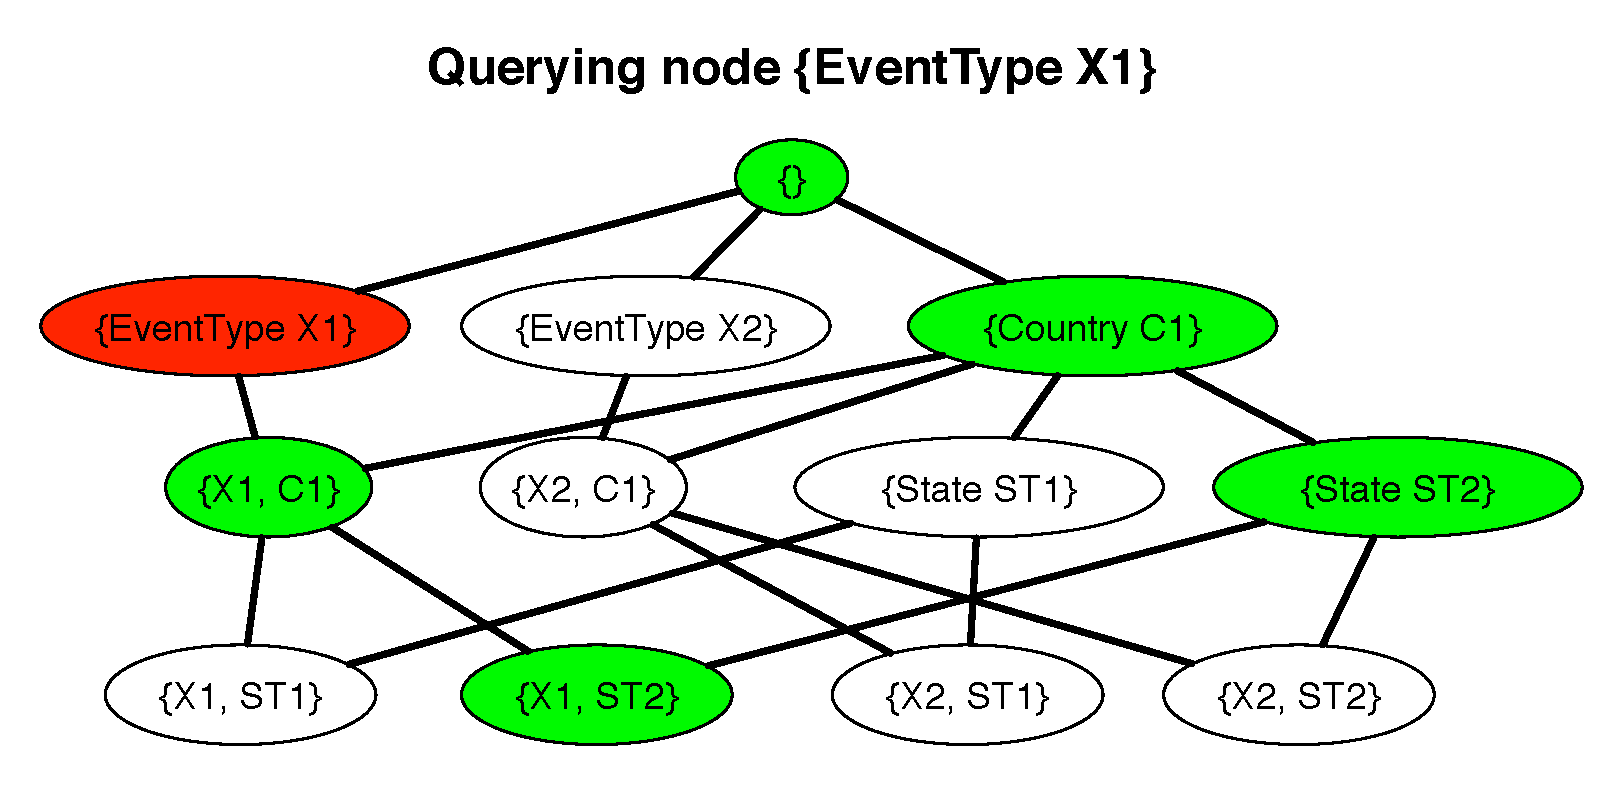
\includegraphics[clip,scale=0.3]{figs/exampleQuery.eps}
	\caption{An example query that extract an entity sample from the red node. The nodes marked with green correspond to the nodes for which indirect entity samples are retrieved.}
	\label{fig:query}
	\vspace{-10pt}
	\end{center}
	\vspace{-5pt}
\end{figure}

We use an example considering the poset in \Cref{fig:eventslattice}, to illustrate these two cases. The example is shown in \Cref{fig:query}. Assume a query $q(k,0)$ issued against node \{EventType X1\}. Assume that the query result contains entities that correspond only to node \{X1,ST2\}. The green nodes in \Cref{fig:query} are nodes for which samples are obtained indirectly without querying them. Notice, that all these nodes are ancestors of \{X1,ST2\}. Analyzing the samples for the different nodes we have:
\squishlist
\item The samples corresponding to nodes \{X1, C1\} and \{X1,ST2\} were obtained by considering their {\em entire population}. The reason is that node \{EventType X1\} is an ancestor of both and the entity population corresponding to it fully contains the populations of both \{X1,C1\} and \{X1,ST1\}. 
\item The samples corresponding to nodes \{ \}, \{Country C1\} and \{State ST2\} were obtained by considering only part of their population. The reason is that the population of node \{EventType X1\} does not fully contain the populations of these nodes. 
\squishend

Samples belonging to both types need to be considered when estimating the gain of a query at a node in $v \in \hierarchy$. To address this issue we merge the extracted entities for each node in $\hierarchy$ into a single sample and treat the unified sample as being extracted from the entire underlying population of the node. As we discuss later in \Cref{sec:solving} we develop querying strategies that traverse the poset $\hierarchy$ in a top-down approach, hence, the number of samples belonging in the first category, i.e., samples retrieved considering the entire population of a node, dominates the number of samples retrieved by considering only part of a node's population. Moreover, it has been shown by Hortal et al.~\cite{hortal2006evaluating} that several of the techniques that can be used to estimate the gain of a query (see \Cref{sec:gainestimators}) are insensitive to differences in the way the samples are aggregated.
\fi
\subsection{Framework Overview}
\label{sec:framework}
We cast the budgeted crowd entity extraction as a multi-round adaptive optimization problem where at each round we solve the following subproblems: 
\squishlist 
\item \textbf{Estimating the Gain for a Query.} For each node in $v \in \hierarchy$, consider the retrieved entities associated with $v$ and estimate the number of new unique entities that will be retrieved if a new query $q^v(k,E)$ is issued at $v$. The query gain is estimated for different query size and exclude list configurations.
\item \textbf{Detecting the Optimal Querying Policy.} Using the gain estimates from the previous problem as input, identify the next (query configuration, node) combination so that the total gain across all rounds is maximized with respect to the given budget constraint. When identifying the next query we do not explicitly optimize for the exclude list to be used. We rather optimize for the exclude list size $l$. Once the size is selected, the exclude list is constructed in a randomized fashion. We elaborate more on this design choice in \Cref{sec:heuristic}.
\squishend
Our proposed framework iteratively solves the aforementioned problems until the entire budget is used. \Cref{fig:framework} shows a high-level diagram of our proposed framework.

\begin{figure}
	\begin{center}
	\includegraphics[clip,scale=0.43]{figs/framework.eps}
	\caption{Framework overview for budgeted entity extraction.}
	\label{fig:framework}
	\end{center}
\end{figure}
%!TEX root = ../crux-sigconf.tex
\section{Budgeted Extraction}
\label{sec:problem}
We now define {\em budgeted crowd entity extraction} over structured domains and present an overview of our framework.
\subsection{Problem Definition}
\label{sec:extraction}
The problem of {\em crowdsourced entity extraction} seeks to extract entities that belong to $\domain$.  For large entity structured domains, one may need to issue a series of entity extraction queries at multiple nodes in  $\hierarchy$---often overlapping with each other---to ensure that the coverage across the domain is maximized. We refer to a series of  generalized $q^v(k,E)$ queries at different nodes $v \in \hierarchy$ as a {\em querying policy}.

Let $\pi$ denote a querying policy. A policy $\pi$ can select a query $q^v(k,E)$ multiple times. Let $C(\pi)$ denote the overall monetary cost of policy $\pi$. We define the gain of $\pi$, denoted by $\uentities(\pi)$, to be the total number of unique entities extracted when following $\pi$. There is a natural trade-off between the gain (i.e., the number of extracted entities) and the cost of policies. 

We require that the user will {\em only} provide a monetary budget $\tau_c$. The poset $\hierarchy$ and the possible query size and exclude list size configurations $(k,l)$ for each node are given as input by the application designer. Our goal is to identify the querying policy that maximizes the number of retrieved entities under the given budget constraint:

\begin{problem}[{\bf Budgeted Crowd Entity Extraction}]\label{prob:budgeted}
Let $\domain$ be an entity domain characterized by a poset $\hierarchy$. For each node $v \in \hierarchy$, let $K^v$ and $L^v$ be the sets of allowed query sizes and exclude list sizes for queries at node $v$. Let $\tau_c$ be a budget on the total cost of issued queries. Find a querying policy $\pi^*$ using queries $q^v(k,E)$ with $k \in K^v$ and $|E| = l \in L^v$ over nodes $v \in \hierarchy$ that maximizes $\uentities(\pi^*)$, the number of unique entities extracted, under the constraint $C(\pi^*) \leq \tau_c$.
\end{problem}
Note that the optimal policy not only specifies the nodes at which queries will be executed but also the size and exclude list of each query. The cost of a querying policy $\pi$ is $C(\pi) = \sum_{q \in \pi} c(q)$, where the cost of each query $q^v$ is defined according to a cost model specified by the user, is easy to compute. However, the number of unique entities extracted by a policy is not known upfront and needs to be estimated as we discuss in \Cref{sec:gainestimators}. Moreover, the problem of finding an optimal querying policy is NP-hard. 

\begin{theorem}[{\bf NP-Hardness}\label{thm:NPH}]
Problem~\ref{prob:budgeted} is NP-hard.
\end{theorem}
The proof is provided 
\iftr in \Cref{sec:prth1}
\fi
\ifpaper in our technical report~\cite{cruxsup} (with all other proofs)
\fi 
and is based on a reduction from the {\em unbounded knapsack} problem. This problem is a variation of the original 0-1 knapsack problem that places no upper bound on the number of copies of each kind of item. 

Finally, computing the total cost of a policy $\pi$ is easy. However, the gain $\uentities(\pi)$ of a policy $\pi$ is unknown as we do not know in advance the entities corresponding to each node in $\hierarchy$, and hence, needs to be estimated (see \Cref{sec:gainestimators}). 

\subsection{Query Response Model}
\label{sec:sampling}
To reason about the occurrence of entities as response to specific queries, we assume that each entity has an {\em unknown popularity value} with respect to crowd workers. Since workers are likely to return different answers based on how the query is phrased, this popularity can be different for different nodes in $\hierarchy$, and thus, is query-dependent. 
Given a query $q^v(1, \emptyset)$, the probability that we get entity $e$ in the result of $q^v$ is simply the popularity value of $e$ divided by the popularity value of all entities $e'$ that also satisfy the same predicate constraints. For example, if there are only two entities $e_1, e_2$ that satisfy the constraints of a query $q_1$, with popularity values $3$ and $2$, then the probability that we get $e_1$ on issuing a query $q_1(1, \emptyset)$ is 3/5. If an exclude list $E$ is specified, then the probability that we get $e \notin E$ is the popularity value of $e$ divided by the popularity values of all entities $e' \notin E$ also satisfying the predicates of $q^v$. 

Since workers are asked to provide a limited number of entities, each query can be viewed as taking a random sample from an unknown population of entities. We refer to the distribution characterizing the popularities of entities in a population as the {\em popularity distribution} of the population. We do not know the popularity distribution in advance; rather we use the samples retrieved by previous queries as a proxy to reason about this distribution. Also, it is not necessary that workers follow the same popularity distribution. Rather, the overall popularity distribution can be seen as an average of the popularity distributions across all workers. 
\iftr
Estimating average statistics across workers is standard practice in crowdsourcing applications~\cite{DasSarma:2016:TGO:2882903.2882953,trushkowsky:2013} since due to the sparsity in the number of answers per worker (especially since workers are fleeting on marketplaces), developing fine-grained models of worker responses can be challenging.
\fi

Estimating the gain of a query $q^v(k,E)$ at a node $v \in \hierarchy$ is equivalent to estimating the number of new entities extracted by taking additional samples from the population of $v$ given all the retrieved entities ({\em running sample}) associated with node $v$. Due to the structure of the poset we may retrieve entities for a node when issuing queries at other nodes. We discuss this form of {\em indirect sampling} in \Cref{sec:indirectsampling}. 

%\iftr
%\stitle{Popularities.} We assume that each underlying entity has a {\em fixed, unknown popularity value} with respect to crowd workers. Given a query $q(1, 0)$, asking for one entity and using an exclude list of size $0$, the probability that we will get entity $e$ that satisfies the constraints specified by $q$ is nothing but the popularity value of $e$ divided by the popularity value of all entities $e'$ that also satisfy the constraints in $q$. As an example, if there are only two entities $e_1, e_2$ that satisfy the constraints specified by a given query $q_1$, with popularity values $3$ and $2$,
%then the probability that we get $e_1$ on issuing a query $q_1(1, 0)$ is 3/5. 
%If an exclude list $S$ is specified, then the probability that we will get an entity $e \notin S$ is the popularity value of $e$ divided by the popularity values of all entities $e' \notin S$ also satisfying the constraints specified by $q$. Note that, we {\bf do not assume that all workers follow the same popularity distribution}. Rather the overall popularity distribution can be seen as an average of the popularity distributions across all workers.
%
%Thus, since workers are asked to provide a limited number of entities as response to a query, each entity extraction query can be viewed as taking a random sample from an unknown population of entities. In the rest of the paper, we will refer to the distribution characterizing the popularities of entities in a population of entities as the {\em popularity distribution} of the population. We note that this is equivalent to the underlying assumption in the species estimation literature~\cite{chao:1992} (\Cref{sec:gainestimators}).
%
%% We assume that the underlying entities exhibit different {\em popularity levels} with respect to crowd workers. These popularity levels can be formally defined using the notion of a probability distribution. In particular, the probability that an entity will appear as part of a query result depends on its {\em popularity} relative to the overall entity population. The popularity of an entity for a query $q$ is defined as the probability that this entity will appear in a query $q(1,0)$, i.e., a query asking for one entity from the population and using an exclude list of size zero. Since workers are asked to provide a limited number of entities as response to a query, each entity extraction query can be viewed as taking a random sample from an unknown population of entities. In the remainder of the paper, we will refer to the distribution characterizing the popularities of entities corresponding to a population as the {\em popularity distribution} of the population. 
%
%Then, estimating the gain of a query $q(k,l)$ at a node $v \in \hierarchy$ is equivalent to estimating the number of new entities extracted by taking additional samples from the population of $v$ given all the retrieved entities by past samples associated with node $v$~\cite{trushkowsky:2013}. 
%
%\stitle{Samples for a Node.} When extracting entities,  the retrieved entities for a node $v$ can correspond to two different kinds of samples: (i) those that were extracted by considering the {\bf entire population} corresponding to node $v$ (ii) and those that we obtained by sampling {\bf only a part of the population} corresponding to $v$. Samples for a node $v$ can be obtained either by querying node $v$ or by indirect information flowing to $v$ by queries at other nodes. We refer to the latter case as {\em dependencies across queries}. 
%\begin{figure}[h]
%	\begin{center}
%	\vspace{-10pt}
%	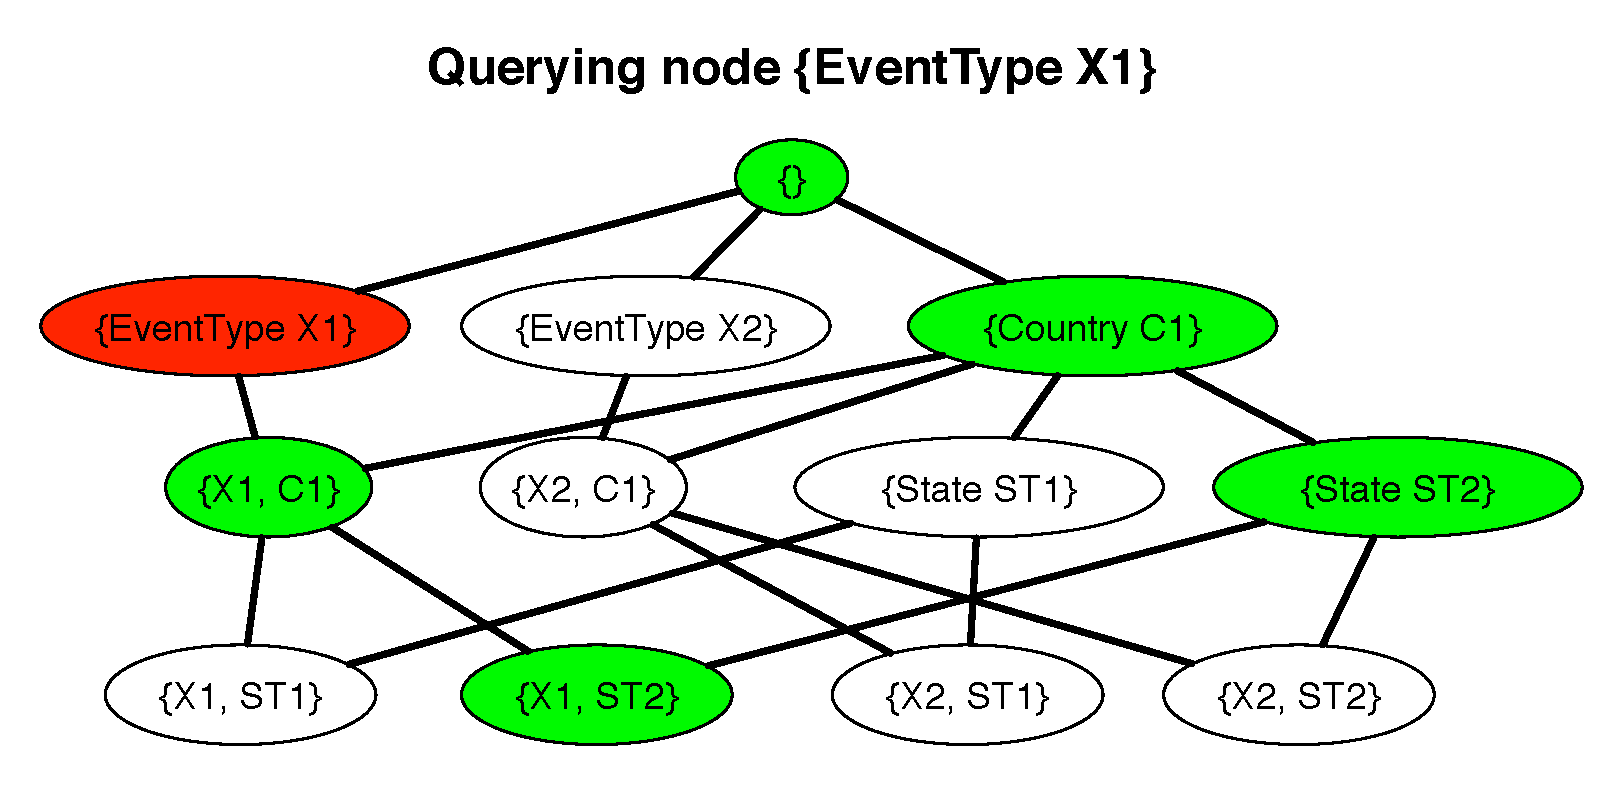
\includegraphics[clip,scale=0.3]{figs/exampleQuery.eps}
%	\caption{An example query that extract an entity sample from the red node. The nodes marked with green correspond to the nodes for which indirect entity samples are retrieved.}
%	\label{fig:query}
%	\vspace{-10pt}
%	\end{center}
%	\vspace{-5pt}
%\end{figure}
%
%We use an example considering the poset in \Cref{fig:eventslattice}, to illustrate these two cases. The example is shown in \Cref{fig:query}. Assume a query $q(k,0)$ issued against node \{EventType X1\}. Assume that the query result contains entities that correspond only to node \{X1,ST2\}. The green nodes in \Cref{fig:query} are nodes for which samples are obtained indirectly without querying them. Notice, that all these nodes are ancestors of \{X1,ST2\}. Analyzing the samples for the different nodes we have:
%\squishlist
%\item The samples corresponding to nodes \{X1, C1\} and \{X1,ST2\} were obtained by considering their {\em entire population}. The reason is that node \{EventType X1\} is an ancestor of both and the entity population corresponding to it fully contains the populations of both \{X1,C1\} and \{X1,ST1\}. 
%\item The samples corresponding to nodes \{ \}, \{Country C1\} and \{State ST2\} were obtained by considering only part of their population. The reason is that the population of node \{EventType X1\} does not fully contain the populations of these nodes. 
%\squishend
%
%Samples belonging to both types need to be considered when estimating the gain of a query at a node in $v \in \hierarchy$. To address this issue we merge the extracted entities for each node in $\hierarchy$ into a single sample and treat the unified sample as being extracted from the entire underlying population of the node. As we discuss later in \Cref{sec:solving} we develop querying strategies that traverse the poset $\hierarchy$ in a top-down approach, hence, the number of samples belonging in the first category, i.e., samples retrieved considering the entire population of a node, dominates the number of samples retrieved by considering only part of a node's population. Moreover, it has been shown by Hortal et al.~\cite{hortal2006evaluating} that several of the techniques that can be used to estimate the gain of a query (see \Cref{sec:gainestimators}) are insensitive to differences in the way the samples are aggregated.
%\fi
\subsection{CRUX Overview}
\label{sec:framework}
CRUX casts the budgeted crowd entity extraction problem as a multi-round adaptive optimization problem where at each round we solve the following subproblems: 
\squishlist 
\item \textbf{Estimating the Gain for a Query}~(\Cref{sec:gainestimators}). For each node $v \in \hierarchy$, consider the retrieved entities associated with $v$ and estimate the number of new unique entities that will be retrieved by a new query $q^v(k,E)$. The query gain is estimated for different query size and exclude list configurations.
\item \textbf{Detecting the Optimal Querying Policy}~(\Cref{sec:solving}). Using the gain estimates from the previous step, identify the query configuration $(k,l,v)$ that maximizes the total gain across all rounds given the budget constraint. When identifying the next query we do not explicitly optimize for the exclude list to be used. We rather optimize for the exclude list size $l$. Once the size is selected, the exclude list is constructed in a randomized fashion. We elaborate more on this in \Cref{sec:config}.
\squishend
CRUX iteratively solves the aforementioned problems until the entire budget is used. 
%\Cref{fig:framework} shows a high-level diagram of our proposed framework.
%
%\begin{figure}
%	\begin{center}
%	\includegraphics[clip,scale=0.43]{figs/framework.eps}
%	\caption{CRUX casts budgeted crowd entity extraction as a multi-round adaptive optimization problem. The main steps per round are shown.}
%	\label{fig:framework}
%	\vspace{-20pt}
%	\end{center}
%\end{figure}
%!TEX root = ../crowd_hierarchies_kdd.tex


\section{Estimating the Gain of Queries}
\label{sec:gainestimators}
Previous work~\cite{trushkowsky:2013} has drawn connections between this problem and the species estimation literature~\cite{chao:1992}. However, the proposed techniques are agnostic to the presence of an exclude-list-based query interface. Moreover, they rely on the presence of a relatively large sample and tend to exhibit negative biases~\cite{hwang:2010, shen:2003}, i.e., they underestimate the expected gain. Negative biases can severely impact entity extraction over large domains since nodes that contain entities that belong in the long tail of the popularity distribution may never be queried as they may be deemed to have zero population. In this section, we first review the existing methodology for estimating the gain of a query. Then we discuss how these estimators can be extended to consider an exclude list. Finally, we propose a new gain estimator for generalized queries $q(k,E)$ that in the presence of little information exhibits lower biases than previous techniques (see \Cref{sec:exps}).

\subsection{Previous Estimators}
\label{sec:prevest}
Consider a specific node $v \in \hierarchy$. Prior work only considers samples retrieved from the entire population associated with $v$ and does not consider an exclude list. Let $Q$ be the set of all existing samples retrieved by issuing queries against $v$ without an exclude list. These samples can be combined into a single sample of size $n = \sum_{q \in Q} {\sf size}(q)$. Let $f_i$ denote the number of entities that appear $i$ times in this unified sample, and let $f_0$ denote the number of unseen entities from the population under consideration. Finally, let $C$ be the population coverage of the unified sample --- that is, this is the fraction of the population covered by the sample.

A new query $q(k,\emptyset)$ at node $v$ can be viewed as increasing the size of the unified sample by $k$. Prior work used techniques from species estimation to estimate the expected number of new entities returned in $q(k,\emptyset)$. Shen et al.~\cite{shen:2003}, derive an estimator for the number of new species $\hat{N}_{Shen}$ that would be found in an increased sample of size $k$. The approach assumes that unobserved entities have equal relative popularity. An estimate of the unique elements found in an increased sample of size $k$ is given by:
\begin{equation}
\label{eq:shen}
\hat{N}_{Shen} = f_0\left( 1 - \left(1 - \frac{1 - C}{f_0}\right)^k\right)
\end{equation}
The second term of Shen's formula corresponds to the probability that at least one unseen entity will be present in a query asking for $k$ more entities. Thus, multiplying this quantity with the number of unseen entities $f_0$ corresponds to the expected number of unseen entities present in the result of a new query $q(k,\emptyset)$.

The quantities $f_0$ and $C$ are unknown and thus need to be estimated considering the entities in the running unified sample. The coverage can be estimated by considering the Good-Turing estimator $\hat{C} = 1 - \frac{f_1}{n}$ for the existing retrieved sample. On the other hand, multiple estimators have been proposed for estimating the number of unseen entities $f_0$. Trushkowsky et al.~\cite{trushkowsky:2013} proposed a variation of an estimator introduced by Chao et al.~\cite{chao:1992} to estimate $f_0$. Nevertheless, the authors argue that the original estimator proposed by Chao performs similarly with their approach when estimating the gain of an additional query $q(k,\emptyset)$. Next, we discuss how one can estimate the return of a query $q(k,E)$ in the presence of an exclude list $E$ of size $l$ and potential negative answers.

%The estimator by Chao~\cite{chao:1992} upon which the authors build has been shown to result in considerable negative bias (i.e., tends to underestimate the parameter) in cases where the number of observed entities from a population represents only a {\em small fraction} of the entire population~\cite{hwang:2010}. Notice, that this assumption holds for crowdsourced entity extraction in a large domain, i.e., we are observing only a small portion of the entire population. To address this problem, Hwang and Shen~\cite{hwang:2010} proposed a regression based technique to estimate $f_0$. This estimator is shown to result in significantly smaller bias and empirically outperforms previously proposed estimators, including the one proposed by Chao, when the ratio of retrieved entities to the entire entity population is small. It also performs comparably to previous estimators when the ratio is larger. Notice that the output of this estimator can also be used as a plug-in quantity in \Cref{eq:shen}. However, both the aforementioned estimators are agnostic to an exclude list and potential negative answers. Next, we discuss how one can estimate the return of a query $q(k,l)$ in the presence of an exclude list of size $l$ and potential negative answers.

%\subsection{Queries With an Exclude List}
%\label{sec:excludelist}
%Consider an exclude list of size $l$. As discussed before an exclude list is a set of entities that correspond to invalid worker answers. Considering an exclude list for a query at a node $v \in \hierarchy$ corresponds to limiting our sampling to a restricted subset of the entity population corresponding to node $v$. In fact, we want to estimate the expected return of a query of size $k$ conditioning on the fact that the entities in the exclude list will not be retrieved by any new sample. The latter corresponds to removing these entities from the population under consideration. Thus, the estimates $\hat{f}_0$ and $\hat{C}$ should be updated before applying \Cref{eq:shen} to compute the expected return of a query of size $k$. This can be done by removing the entities included in the exclude list from the running sample for node $v$, recomputing the entity counts $f_i$ and following the techniques presented above for computing the updated estimates for $\hat{f}_0$ and $\hat{C}$. This approach requires that the exclude list is known in advance. To construct an exclude list one can follow a randomized approach, where $l$ of the retrieved entities are included in the list uniformly at random. The generated list can be used to update the frequency counts $f_i$ and estimate the gain of the query. Bootstrapping can also be used to obtain improved estimates.

\subsection{Exclude Lists and Negative Answers}
\label{sec:excludelist}
An exclude list $E$ of size $l$ for a query at a node $v \in \hierarchy$ is a set of entities that correspond to invalid worker answers. Effectively it limits sampling to a restricted subset of the entity population corresponding to node $v$ and corresponds to estimating the expected return of a query of size $k$ conditioning on the fact that the entities in the exclude list will not be retrieved by any new sample. The estimates $\hat{f}_0$ and $\hat{C}$ should be updated before applying \Cref{eq:shen} by removing the entities included in the exclude list from the running sample for node $v$. This approach requires that the exclude list is known in advance. To construct an exclude list one can follow a randomized approach, where $l$ of the retrieved entities are included in the list uniformly at random. The generated list can be used to update the frequency counts $f_i$ and estimate the gain of the query. Bootstrapping can also be used to obtain improved estimates. 

We follow a randomized approach as a deterministic construction of $E$ that picks the {\em l-most} popular items in the running sample is very sensitive to the {\em observed popularity distribution}. When the number of observed entities corresponds to a small portion of the entire population - as in the scenarios we consider in this paper - the individual entity popularity estimates tend to be very noisy.  We empirically observed that a deterministic construction of a limited size exclude list, especially during early queries, leads to poor popularity estimates. Thus, we choose to follow a randomized approach.

Next, we study the effect of {\em negative answers} on estimating the gain of future queries. It is possible to issue a query at a specific node $v \in \hierarchy$ and receive no entities, i.e., we receive a negative answer. This is an indication that the underlying entity population of $v$ is empty. In such a scenario, we assign the expected gain of future queries at $v$ and all its descendants to zero. Another type of negative answer corresponds to issuing a query at an ancestor node $u$ of $v$ and receiving no entities for $v$. In this case, we do not update our estimates for node $u$ as entities from other descendants of $u$ may be more popular than entities associated with $u$.

\subsection{Direct Gain Estimation}
\label{sec:newestim}
The techniques reviewed in \Cref{sec:prevest} result in negative bias when the number of observed entities from a population represents only a {\em small fraction} of the entire population~\cite{hwang:2010, shen:2003}. This holds for the large and sparse domains we consider in this paper. To address this problem, Hwang and Shen~\cite{hwang:2010} proposed a regression based technique to estimate $f_0$ and show that it results in smaller biases. However, estimating the total gain of a query requires coupling this new estimator with \Cref{eq:shen}, thus, it may still exhibit negative bias. To eliminate negative bias, we propose a direct estimator for the gain of generalized queries $q(k,E)$ without using \Cref{eq:shen}. We build upon the techniques in~\cite{hwang:2010} and use a regression based technique that captures the structural properties of the expected gain function. \ifpaper The proofs for the results below can be found in the extended version of this paper~\cite{crowdgatherfull}. \fi

Let $S$ denote the total number of entities in the population under consideration and $p_i$ the abundance probability (i.e., popularity) of entity $i$. Given a sample of size $n$ from the population, define $K(n)$ to be $K(n) = \frac{\sum_{i=1}^S (1-p_i)^n}{\sum_{i=1}^S p_i(1-p_i)^{n-1}}$. First, we focus on queries without an exclude list. Later we relax this discuss queries with exclude lists. We have the following theorem on query gain:

\vspace{-5pt}\begin{theorem}
\label{newgain}
Given a node $v \in \hierarchy$ and a corresponding entity sample of size $n$, let $f_1$ and $f_2$ denote the number of entities that appear exactly once (i.e., singletons) and exactly twice respectively. Let $G$ denote the number of new items retrieved by a query $q(m,\emptyset)$. We have that:

\vspace{-10pt}\begin{equation}
\label{eq:dirgain}
G = \frac{1}{(1 + \frac{K^{\prime}}{n+m})}(K\frac{f_1}{n} - K^{\prime}\frac{f_1(1-\frac{1}{n}2\frac{f_2}{f_1})^m}{n+m})
\end{equation}
where $K = K(n)$ and $K^{\prime} = K(n+m)$.
\end{theorem}
\iftr
\begin{proof}
To derive the new estimator we make used of the generalized jackknife procedure for species richness estimation~\cite{heltshe1983estimating}. Given two (biased) estimators of $S$, say $\hat{S}_1$ and $\hat{S}_2$, let $R$ be the ratio of their biases:
\begin{equation}
R = \frac{E(\hat{S}_1) - S}{E(\hat{S}_2) - S}
\end{equation}
By the generalized jackknife procedure, we can completely eliminate the bias resulting from either $\hat{S}_1$ or $\hat{S}_2$ via
\begin{equation}
S = G(\hat{S}_1, \hat{S}_2) = \frac{\hat{S}_1 - R\hat{S}_2}{1 - R}
\label{eq:jknife}
\end{equation}
provided the ratio of biases $R$ is known. However, $R$ is unknown and needs to be estimated. 

Let $D_n$ denote the number of unique entities in a unified sample of size $n$. We consider the following two biased estimators of $S$: $\hat{S_1} = D_n$ and $\hat{S}_2 = \sum_{j=1}^n D_{n-1}(j)/n = D_n - f_1/n$ where $D_{n-1}(j)$ is the number of species discovered with the $j$th observation removed from the original sample. Replacing these estimators in \Cref{eq:jknife} gives us:
\begin{equation}
S = D_n +\frac{R}{1-R}\frac{f_1}{n}
\end{equation}
Similarly, for a sample of increased size $n+m$ we have:
\begin{equation}
S = D_{n+m} +\frac{R^{\prime}}{1-R^{\prime}}\frac{f^{\prime}_1}{n+m}
\end{equation}
where $R^{\prime}$ is the ratio of the biases and $f^{\prime}_1$ the number of singleton entities for the increased sample. Let $K = \frac{R}{1-R}$ and $K^{\prime} = \frac{R^{\prime}}{1-R^{\prime}}$. Taking the difference of the previous two equations we have:
\begin{equation}
D_{n+m} - D_{n} = K\frac{f_1}{n} - K^{\prime}\frac{f^{\prime}_1}{n+m}
\end{equation}
Therefore, we have:
\begin{equation}
\label{eq:new}
G = K\frac{f_1}{n} - K^{\prime}\frac{f^{\prime}_1}{n+m}
\end{equation}
We need to estimate $K$, $K^{\prime}$ and $f^{\prime}_1$. We start with $f^{\prime}_1$, which denotes the number of singleton entities in the increased sample of size $n+m$. Notice, that $f^{\prime}_1$ is not known since we have not obtained the increased sample yet, so we need to express it in terms of $f_1$, i.e., the number of singletons, in the running sample of size $n$. We have:
\begin{equation}
f^{\prime}_1 = G + f_1 - f_1^c
\end{equation}
where $f_1^c$ denotes the number of old singleton entities from the sample of size $n$ that appeared in the additional query of size $m$. Let $E_1$ denote the set of singleton entities in the old sample of size $n$. We approximate $f_1^c$ by its expected value:
\begin{equation}
\hat{f}_1^c = \sum_{e \in E_1} \Pr[\mbox{e appears in query of size $m$}]
\end{equation}
We compute the probability of an old singleton entity appearing in an additional query as follows. Let $p_e$ denote the popularity of entity $e$. As described before, an additional query of size $m$ corresponds to taking a sample of size $m$ from the underlying entity population without replacement. However, $m$ is significantly smaller compared to the size of the underlying population, thus, we can consider a that taking a sample of size $m$ corresponds to taking a sample {\em with replacement}. Following this we have that:
\begin{equation}
\Pr[\mbox{e appears in query of size $m$}] = 1 - (1-p_e)^m
\end{equation}
Following a standard approach in the species estimation literature we assume that the popularity of retrieving a singleton entity again is the same for all singleton entities. This popularity can be computed using the corresponding Good-Turing estimator considering the running sample. We have:
\begin{equation}
\forall e \in E_1, p_e = p_1 = \hat{\theta}(1) = \frac{1}{n}2\frac{f_2}{f_1}
\end{equation}
where $f_2$ is the number of entities that appear twice in the sample and $f_1$ is the number of singletons. 
Eventually we have that:
\begin{equation}
\hat{f}_1^c = f_1(1 - (1-p_1)^m)
\end{equation}
and
\begin{equation}
f^{\prime}_1 = G + f_1(1-p_1)^m
\end{equation}
Replacing the last equation in \Cref{eq:new} we have:
\begin{align}
&G = K\frac{f_1}{n} - K^{\prime}\frac{G + f_1(1-p_1)^m}{n+m} \nonumber \\
&G = K\frac{f_1}{n} - K^{\prime}\frac{G}{n+m} - K^{\prime}\frac{f_1(1- P)}{n+m} \nonumber \\
&G(1 + \frac{K^{\prime}}{n+m}) = K\frac{f_1}{n} - K^{\prime}\frac{f_1(1- P)}{n+m} \nonumber \\
&G = \frac{1}{(1 + \frac{K^{\prime}}{n+m})}(K\frac{f_1}{n} - K^{\prime}\frac{f_1(1-p_1)^m}{n+m}) \nonumber
\end{align}
\end{proof}
\fi
All quantities apart from $K$ and $K^{\prime}$ in \Cref{eq:dirgain} are known. The value of $K$ can be estimated using the regression approach introduced by Hwang and Shen~\cite{hwang:2010}. \iftr From the Cauchy-Schwarz inequality we have that:
\begin{equation}
K = \frac{\sum_{i=1}^S (1-p_i)^n}{\sum_{i=1}^S p_i(1-p_i)^{n-1}} \geq \frac{(n-1)f_1}{2f_2}
\end{equation}
This can be generalized to:
\begin{equation}
K=\frac{nf_0}{f_1} \geq \frac{(n-1)f_1}{2f_2} \geq \frac{(n-2)f_2}{3f_3} \geq \dots
\end{equation}
Let $g(i) = \frac{(n-i)f_i}{(i+1)f_{i+1}}$. From the above we have that the function $g(x)$ is a smooth monotone function for all $x \geq 0$. Moreover, let $y_i$ denote a realization of $g(i)$ mixed with a random error. Hwang and Shen how one can use an exponential regression model to estimate $K$. The proposed model corresponds to:
\begin{equation}
y_i = \beta_0\exp(\beta_1i^{\beta_2}) + \epsilon_i
\end{equation}
where $i = 1, \dots, n-1$, $\beta_0 > 0$, $\beta_1 < 0$, $\beta_2 >0$ and $\epsilon_i$ denotes random errors. It follows that $K = \beta_0$. \fi
To estimate the value of $K^{\prime}$ for an increased sample of size $n+m$, we first show that $K$ increases monotonically as the size of the running sample increases. 

\begin{lemma}
\label{monotonicity}
The function $K(n) = \frac{\sum_{i=1}^S (1-p_i)^n}{\sum_{i=1}^S p_i(1-p_i)^{n-1}}$ increases monotonically, i.e., $K(n+m) \geq K(n), \forall n,m > 0$.
\end{lemma}
\iftr
\begin{proof}
In the remainder of the proof we will denote $K(n+m)$ as $K^{\prime}$. By definition we have that $K = \frac{\sum_{i=1}^S (1-p_i)^n}{\sum_{i=1}^S p_i(1-p_i)^{n-1}}$ and $K^{\prime} = \frac{\sum_{i=1}^S (1-p_i)^{n+m}}{\sum_{i=1}^S p_i(1-p_i)^{n+m-1}}$. We want to show that:

{\small
\begin{align}
&\frac{\sum_{i=1}^S (1-p_i)^{n+m}}{\sum_{i=1}^S p_i(1-p_i)^{n+m-1}} \geq \frac{\sum_{i=1}^S (1-p_i)^n}{\sum_{i=1}^S p_i(1-p_i)^{n-1}} \nonumber \\
&\sum_{i=1}^S (1-p_i)^{n+m}\sum_{j=1}^S p_j(1-p_j)^{n-1} \geq \sum_{i=1}^S p_i(1-p_i)^{n+m-1}\sum_{j=1}^S (1-p_j)^n\nonumber \\
&\sum_{i,j:i\prec j}[(1-p_i)^{n+m}p_j(1-p_j)^{n-1} - p_i(1-p_i)^{n+m-1}(1-p_j)^n + \nonumber \\
& + (1-p_j)^{n+m}p_i(1-p_i)^{n-1} - p_j(1-p_j)^{n+m-1}(1-p_i)^n] \geq 0 \nonumber \\
%&\sum_{i,j:i\prec j}[(1-p_i)^{n}(1-p_j)^{n-1}p_j((1-p_i)^{m} - (1-p_j)^{m})  + \nonumber \\
%& - (1-p_j)^{n}p_i(1-p_i)^{n-1}((1-p_i)^{m} - (1-p_j)^{m}) \geq 0 \nonumber \\
&\sum_{i,j:i\prec j}[(1-p_i)^{n-1}(1-p_j)^{n-1}(p_j-p_i)((1-p_i)^{m} - (1-p_j)^{m}) \geq 0
\end{align}}

But the last inequality always holds since each term of the summation is positive. In particular, if $p_j \geq p_i$ then
also $1-p_i \geq 1-p_j$ and if $p_j \leq p_i$ then $1-p_i \leq 1-p_j$.
\end{proof}
\fi
Given the monotonicity of function $K$, we model $K$ as a generalized logistic function of the form $K(x) = \frac{A}{1+exp(-G(x-D))}$. As we observe samples of different sizes for different queries we estimate $K$ as described above and therefore we observe different realizations of $f(\cdot)$. Thus, we can learn the parameters of $f$ and use it to estimate $K^{\prime}$. In the presence of an exclude list of size $l$ we follow the approach described in \Cref{sec:excludelist} to update the quantities $f_i$ used in the analysis above. 

%\subsection{Negative Answers and Gain Estimation}
%\label{sec:neg}
%Next, we study the effect of {\em negative answers} on estimating the gain of future queries. It is possible to issue a query at a specific node $v \in \hierarchy$ and receive no entities, i.e., we receive a negative answer. This is an indication that the underlying entity population of $v$ is empty. In such a scenario, we assign the expected gain of future queries at $v$ and all its descendants to zero. 
%
%Another type of negative answer corresponds to the scenario where we issue a query at an ancestor node $u$ of $v$ and receive no entities associated with $v$ but received some entities for $u$. Notice, that in this case, we do not have enough information to update our estimates for node $u$. The reason is that due to the restricted query size entities from other descendants of $u$ may be more popular with respect to the popularity distribution of $u$.
%!TEX root = ../crowd_hierarchies_kdd.tex


\section{Discovering Querying Policies}
\label{sec:solving}
We now turn our attention to the core component of CRUX and introduce a heuristic multi-round adaptive optimization algorithm for identifying querying strategies that maximize the total gain across all rounds under the given budget constraints. At each round we assume oracle access to a gain estimator for any generalized query $q^v(k,E)$. Such oracles can be constructed using the techniques introduced in the previous section. The gain of each query can be viewed as a random variable. By issuing a query we get to observe the value of this random variable and using the previous observations we need to decide which query to issue. Given the above, our framework builds upon ideas from the multi-armed bandit literature~\cite{Auer:2003,EvenDar06actionelimination}. Before presenting our framework we discuss some challenges associated with this adaptive optimization problem.

\squishlist
\item The first challenge is that the number of nodes in $\hierarchy$ is exponential in the number of attributes $\attributes$ describing the domain of interest. Querying every possible node to estimate its expected return for different queries $q^v(k,E)$ is prohibitively expensive. That said, typical budgets do not allow algorithms to query all nodes in the hierarchy, so this intractability may not hurt us all that much. For example, we keep estimates for each of the nodes for which at least one entity has been retrieved.
\item The second challenge is balancing the tradeoff between {\em exploitation} and {\em exploration}~\cite{Auer:2003}. The first refers to querying nodes for which sufficient entities have been retrieved, and hence, we have an accurate estimate for their expected gain; the latter refers to exploring nodes to avoid myopic policies.
\item The last challenge is optimizing over the exclude list to be used in queries. Optimizing over all potential exclude lists (i.e., considering all potential subsets of observed entities to be added in the list) leads to an exponential explosion of the query space. As we discuss next, optimizing over all potential query configurations $(k,l,v)$ can limit the query space significantly.
\squishend

\subsection{Optimizing over Query Configurations}
\label{sec:config}
Instead of optimizing over all potential queries $q^v(k,E)$, we optimize over all potential query configurations $(k,l,v)$. That is, we do not optimize directly for the exclude list to be used in a further query but rather for the size $l$ of it. Once we decide on $l$ the exclude list $E$ can be constructed following a randomized approach, where $l$ of the retrieved entities are included in the list uniformly at random. We follow a randomized approach since a deterministic construction of $E$ that picks the {\em l-most} popular items in the running sample is very sensitive to the {\em observed popularity distribution}. When the number of observed entities corresponds to a small portion of the entire population -- as in the scenarios we consider in this paper -- the individual entity popularity estimates tend to be noisy.  We empirically observed that a deterministic construction of a limited size exclude list, especially during early queries, leads to poor popularity estimates. Thus, we follow a randomized approach. Below we denote a query configuration $(k,l,v)$ and a query $q^v(k,E)$ with $|E| = l$ using the same symbol $q$ for convenience. Given $l$ we construct $E$ following the aforementioned approach.

Given the above, we need to estimate the gain for a query configuration $(k,l,v)$ instead of a query $q^v(k,E)$. When $l = 0$, i.e., $E = \emptyset$, then we can directly use the techniques introduced in \Cref{sec:gainestimators}. When $l \neq 0$, we use the following approach. We generate multiple instances of $q^v(k,E)$ queries following the configuration $(k,l,v)$ and use the techniques from \Cref{sec:gainestimators} to estimate the expected gain of ite. The exclude list of each query is generated following the randomized approach described above. Finally, we estimate the expected gain of configuration $(k,l,v)$ by considering the average gain of all generated query instances. The variance of the gain is also considered for determining an upper bound on the gain of the query configuration $(k,l,v)$ as described next.

\subsection{Balancing Exploration and Exploitation}
\label{sec:balancing}
In the previous subsection we described how we can estimate the expected gain of a query configuration $(k,l,v)$. However, this estimate is based on a rather small sample of the underlying population. Thus, exploiting this information at every round may lead to suboptimal decisions. Because of this we need to balance the trade-off between exploiting query configurations for which the estimated gain is high and configurations that have not been selected many times. Formally, the latter corresponds to upper-bounding the expected gain of each query configuration with a {\em confidence interval} that depends on both the variance of the expected gain and the number of times a query has been issued~\cite{Auer:2003}.

Next we will use $q$ to denote a query configuration $(k,l,v)$. Let $r(q)$ denote the expected gain of $q$. This is an estimate of the true gain $r^*(q)$. Moreover, let $\sigma(q)$ be an error component on the gain of configuration $q$ chosen such that $r(q) - \sigma(q) \leq r^*(q) \leq r(q) + \sigma(q)$ with high probability. The parameter $\sigma(q)$ should take into account both the {\bf empirical variance} of the expected gain as well as our {\bf uncertainty} about the gain of query configuration $q$ if $q$ has been chosen only a few times. Given the quantities $r(q)$ and $\sigma(q)$, we assign a score to each configuration by considering a linear function of the quantity $r(q) + \sigma(q)$. This score prioritizes exploration when the variance or our uncertainty is high, and thus, we could potentially discover a profitable new configuration, and exploitation when the estimated gain is high. Next, we discuss how we set the quantity $\sigma(q)$.

We proceed in rounds and at each round select a query configuration $q$. Let $n_{q,t}$ be the number of times we have chosen $q$ by round $t$, and let $v_{q,t}$ denote the maximum value between some constant (e.g., $0.01$) and the empirical variance for the gain for $q$ at round $t$. The latter can be computed using bootstrapping over the retrieved sample and applying the estimators presented in \Cref{sec:gainestimators} over these bootstrapped samples. Several techniques have been proposed in the multi-armed bandits literature to compute the parameter $\sigma(q)$~\cite{teytaud:inria-00173263}. Teytaud et al.~\cite{teytaud:inria-00173263} showed that techniques considering both the variance and the number of times an action, here a query, has been chosen tend to outperform other proposed methods. Based on this observation, we choose to use the following formula for sigma:
\begin{equation}
\label{eq:upper}
\sigma(q,t) = \sqrt{\frac{v_{q,t}\cdot\log(t)}{n_{q,t}}}
\end{equation}

\subsection{A Multi-Round Querying Policy Algorithm}
\label{sec:heuristic}
We now introduce a multi-round algorithm for solving the budgeted entity enumeration problem. An overview of our multi-round optimization algorithm is shown in Algorithm~\ref{algo:overall}. The algorithm takes as input the poset $\hierarchy$ describing the extraction domain, a set $K$ of valid query size assignments, a set $L$ of valid exclude list size assignments and a budget $\tau_c$. The algorithm also assumes access to an oracle providing the values $r(q)$ and $\sigma(q,t)$ - $t$ denotes the round count -  which characterize the upper gain of a query configuration $q$ and an oracle providing the cost $c(q)$ of $q$. Finally, the algorithm has access to the method ${\sf ActiveQueryConf}$ (see \Cref{sec:badactions}) which determines the possible query configurations to be considered at each round.

\begin{algorithm}[h]
\small\caption{Multi-round Extraction Algorithm}
\label{algo:overall}
\begin{algorithmic}[1]
\STATE {\bf Input:} $\hierarchy$: the hierarchy describing the entity domain; $K$: set of valid query size assignments; $L$: set of valid exclude-list size assignments; $\tau_c$: budget; $r,\sigma$: value oracle access to upper-bounded gain for different query configurations; $c$: value oracle access to the query configuration costs;
\STATE {\bf Output:} $\uentities$: a set of extracted distinct entities;
\STATE $\uentities \leftarrow \{\}$
\STATE $t \leftarrow 1$ /* Initialize round counter */
\STATE ${\sf Rembudget} \leftarrow \beta_c$ /* Initialize remaining budget */
\STATE $\mathcal{Q} \leftarrow$ {\sf ActiveQueryConf($\hierarchy$, $\emptyset$, NULL $K$, $L$, $t$)} /* Initialize active query configurations */
\WHILE {${\sf Rembudget} > 0$ and $\mathcal{Q} \neq \{\}$}
	\STATE $q^* \leftarrow \arg\max_{q \in {\mathcal{Q}}} \frac{r(q)+\sigma(q,t)}{c(q)}$ s.t. ${\sf Rembudget} - c(q^*) >0$
	\IF {$q^*$ is NULL }
		\STATE break;
	\ENDIF
	\STATE ${\sf Rembudget} \leftarrow {\sf Rembudget} - c(q^*)$ /* Update budget */
	\STATE Given configuration $q^* = (k^*,l^*,v^*)$ generate an exclude list $E$ such that $|E| = l^*$; 
	\STATE Issue query $q^{v^{*}}(k^*,E)$
	\STATE $E \leftarrow$ entities extracted by query $q^{v^{*}}(k^*,E)$
	\STATE $\uentities \leftarrow \uentities \cup E$ /* Update unique entities */
	\STATE $\mathcal{Q} \leftarrow$ {\sf ActiveQueryConf($\hierarchy$, $\mathcal{Q}$, $v^*$, $K$, $L$, $t$)} /* Update active queries */
	\STATE $t \leftarrow t + 1$ /* Increase round counter */
\ENDWHILE
\RETURN $\uentities$
\end{algorithmic}
\end{algorithm}

Our multi-round extraction algorithm proceeds as follows: First it initializes the set $\uentities$ of extracted entities, the round count $t$, the remaining budget ${\sf Rembudget}$ and the set of candidate queries $\mathcal{Q}$ (i.e., query configurations to be considered) at the first round (Ln.3-6). Then it proceeds in rounds and iteratively selects one query configuration to be used until the total budget is utilized or the set of candidate queries is empty (Ln. 7). At each round our algorithm performs the following steps. It first detects a configuration in $\mathcal{Q}$ that maximizes the score quantity $\frac{r(q) + \sigma(q,t)}{c(q)}$ under the constraint that the cost $c(q)$ is less or equal to the remaining budget (Ln. 8). If no such configuration exists the algorithm terminates (Ln. 9-10). Otherwise, the algorithm proceeds by executing a query corresponding to the selected configuration $q^*$, updates the set of extracted entities, the remaining budget, the set of active queries, and the round counter (Ln. 11 - 17). Finally, Algorithm 1 returns the set of distinct entities extracted (Ln. 18). 

\vspace{2pt}\noindent\textbf{Discussion.} The reason we chose $\frac{r(q) + \sigma(q,t)}{c(q)}$ as the assigned query configuration score is due to the presence of a budget and the connection between budgeted crowdsourced entity extraction and knapsack style problems. Finally, method ${\sf ActiveQueryConf}$ is used to restrict the set of candidate query configurations considered by our algorithm. As discussed before the size of $\hierarchy$ is exponential to the values of attributes describing it, and thus, considering all possible configurations $(k,l)$ for the different nodes of $\hierarchy$ can be prohibitively expensive. 

\subsection{Updating the Set of Actions}
\label{sec:badactions}
We now introduce an algorithm for effectively limiting the number of query configurations considered at each round of Algorithm \ref{algo:overall}. To do so we exploit the structure of poset $\hierarchy$ and the gain estimates for different query configurations $q = (k,l,v)$. Let $\mathcal{Q}$ denote the set of candidate (or active) query configurations to be considered. We propose an algorithm that {\bf adds} configurations to $\mathcal{Q}$ by traversing the input poset in a top-down manner. These configurations $(k,l,v)$ are associated with nodes $v$ that are {\em direct descendants} of already queried nodes. 

The reason we adopt a top-down traversal is two-fold: (i) Due to the hierarchical structure of the poset nodes at higher levels of the poset correspond to larger populations of entities. Therefore, issuing queries at these nodes can potentially result in a larger number of extracted entities. Hence, traversing the poset in a top-down manner allows us to detect sparsely populated areas of the poset and prune futile queries. (ii)According to our cost model assumption, issuing queries at higher-level nodes (i.e., less specialized queries) is cheaper. Therefore, the gain to cost ratio can be larger for queries that correspond to higher-level nodes of the poset.

As mentioned above the number of nodes in $\hierarchy$ can be prohibitively large, therefore we also {\bf remove} any {\em bad query configurations} from set $\mathcal{Q}$. A configuration $q$ is defined to be bad at round $t$ when $r(q) + \sigma(q,t) < \max_{q^{\prime} \in \mathcal{Q}} (r(q^{\prime}) - \sigma(q^{\prime},t))$. Intuitively, this states that we do not need to consider a configuration as long as there exists another one such that the upper-bounded gain of the former is lower than the lower bounded gain of the latter. This technique is also adopted in multi-armed bandits to limit the number of actions considered by the algorithm~\cite{EvenDar06actionelimination}. 

An overview of our algorithm is shown in Algorithm~\ref{algo:updateactions}. This also implements the method ${\sf ActiveQueryConf}$ introduced above. The algorithm takes as input the poset $\hierarchy$ describing the extraction domain, a set $K$ of valid query size assignments, a set $L$ of valid exclude list size assignments and a budget $\tau_c$. The algorithm also assumes access to an oracle providing the values $r(q)$ and $\sigma(q,t)$ - $t$ denotes the round count -  which characterize the upper gain of a query $q$ and an oracle providing the cost $c(q)$ of a query $q$. Finally, the algorithm has access to the method ${\sf ActiveQuerySet}$ (see \Cref{sec:badactions}) which determines the possible queries to be considered at each round.

An overview of our algorithm for determining the set of active queries to be considered at each round is shown in Algorithm~\ref{algo:updateactions}. This algorithm implements the method ${\sf ActiveQuerySet}$ introduced above. The method takes as input the poset $\hierarchy$ describing the extraction domain, a set $K$ of valid query size assignments, a set $L$ of valid exclude list size assignments, the running set $\mathcal{Q}_{old}$ of active query configurations, the node $v^*$ associated with the last query issued against the crowd, and the running round $t$. The algorithm also assumes access to an oracle providing the values $r(q)$ and $\sigma(q,t)$  which characterize the upper gain of a query configuration $q$.

The algorithm proceeds as follows: If the running set of active queries is empty (Ln. 3), i.e., if we have issued no queries previously, the set of active query configurations is initialized to contain all potential configurations $(k,l)$ associated with the root of the poset $\hierarchy$ (Ln. 6). Otherwise, the algorithm first adds all query configurations associated with the direct descendants of node $v^*$ to the running set $\mathcal{Q}_{old}$ (Ln. 9 - 11) and then removes any bad query configurations from the new set $\mathcal{Q}_{new}$ (Ln.13-16). The algorithm terminates by returning the set $\mathcal{Q}_{new}$.

\begin{algorithm}[h]
\small\caption{UpdateActionSet}
\label{algo:updateactions}
\begin{algorithmic}[1]
\STATE {\bf Input:} $\hierarchy$: the hierarchy describing the entity domain; $\mathcal{Q}_{old}$: the running set of active query configurations; $v^*$: the node in $\hierarchy$ associated with the last query; $K$: set of valid query size assignments; $L$: set of valid exclude-list size assignments; $t$: running round counter; $r,\sigma$: value oracle access to upper-bounded gain for different query configurations;
\STATE {\bf Output:} $\mathcal{Q}_{new}$: the updated set of active query configurations;
\IF {$\mathcal{Q}_{old}$ is empty} 
	\STATE \textbf{/* Initialize Set of Active Query Configurations */}
	\STATE /* Populate ${\mathcal{Q}_{new}}$ with all possible $(k,l)$ configuration for the root of $\hierarchy$. */
	\STATE ${\mathcal{Q}_{new}} \leftarrow \bigcup_{k \in K \times l \in L} \{ (k,l,root) \}$
\ELSE
	\STATE \textbf{/* Extend Set of Active Query Configurations */}
	\STATE $\mathcal{Q}_{new} \leftarrow \mathcal{S}_{old}$
	\FORALL{$d \in ${\sf ~Set of Direct Descendant Nodes of $v^*$}}
	\STATE $\mathcal{Q}_{new} \leftarrow \mathcal{Q}_{new} \cup \bigcup_{k \in K \times l \in L} \{(k,l,d)\}$
	\ENDFOR
	\STATE \textbf{/* Remove Bad Query Configurations*/}
	\STATE /* Find maximum lower-bounded gain over all $q$ in $\mathcal{Q}_{new}$*/
	\STATE $\psi \leftarrow \max_{q^{\prime} \in \mathcal{Q}_{new}} (r(q^{\prime}) - \sigma(q^{\prime},t))$  
	\STATE $\mathcal{B} \leftarrow$ All configurations $q$ in $\mathcal{Q}_{new}$ with $r(q) + \sigma(q,t) < \psi$
	\STATE $\mathcal{Q}_{new} \leftarrow \mathcal{Q}_{new} \setminus \mathcal{B}$
\ENDIF 
\RETURN $\mathcal{Q}_{new}$
\end{algorithmic}
\end{algorithm}
\vspace{-5pt}

%!TEX root = ../crux.tex


\section{Experimental Evaluation}
\label{sec:exps}
We present an empirical evaluation of CRUX on both real and synthetic datasets. First, we discuss the experimental methodology, then we describe the data and results showing the effectiveness CRUX on crowdsourced entity extraction. The evaluation is performed on an Intel(R) Core(TM) i7 3.7 GHz 32GB machine; all algorithms are implemented in Python 2.7. 

\subsection{Experimental Setup}
\label{sec:expsetup}
\noindent\textbf{Gain Estimators.} We evaluate the gain estimators below:
\squishlist
\item {\bf Chao92Shen}, combines the methodology proposed by Chao~\cite{chao:1992} with Shen's formula, i.e., \Cref{eq:shen}.
\item {\bf HwangShen}, combines the regression-based approach proposed by Hwang and Shen~\cite{hwang:2010} with Shen's formula. 
\item {\bf NewRegr}, our new technique proposed in \Cref{sec:newestim}.
\squishend
All estimators are coupled with bootstrapping to estimate the gain variance used to upper bound the return of a query as shown in \Cref{sec:balancing}.

\noindent\textbf{Entity Extraction Algorithms.} We evaluate the following algorithms for crowdsourced entity extraction:
\squishlist
\item {\bf Rand}, executes random queries until all the available budget is used. It selects a random node from $\hierarchy$ and a random query configuration $(k,l)$ valid with the $k$, $l$ input. \iftr We expect Rand to be effective for extracting entities in small and dense data domains that do not have many sparsely populated nodes. \fi
\item {\bf RandL}, same as Rand but only executes queries {\em at the leaf nodes} of $\hierarchy$ until all the available budget is used.  \iftr We expect RandL to be effective for {\em shallow} data domains when the majority of nodes corresponds to leaf nodes. Like Rand, the performance of RandL is expected to be reasonable for small and dense data domains without sparsely populated nodes.\fi
\item {\bf BFS}, performs a breadth-first traversal of $\hierarchy$, executing one query at each node. The query configuration is randomly selected all valid combinations. \iftr It also takes into account the structure of the input domain but is agnostic to sparsely populated nodes of the input $\hierarchy$. \fi
\item {\bf RootChao}, corresponds to the entity extraction scheme of Trushkowsky et al.~\cite{trushkowsky:2013} that uses Chao92Shen to measure the gain of an additional query. RootChao is agnostic to the structure of the input domain, thus, equivalent to issuing queries only at the root node of $\hierarchy$. Since the authors only propose a pay-as-you-go scheme, we coupled this algorithm with Alg.~\ref{algo:overall} to optimize for the input budget constraint. We allow the algorithm to consider different query configurations $(k,l)$ but restrict the possible queries to the root node.
\item {\bf GSChao, GSWang, GSNewR}, are different variations of CRUX. These algorithms correspond to our proposed graph search querying policy algorithm (\Cref{sec:heuristic}) coupled with Chao92Shen, HwangShen and NewRegr respectively.
\item {\bf GSExact}, is used as a near-optimal, omniscient baseline that allows us to see how far off our algorithms are from an algorithm with perfect information. We combine the algorithm proposed in \Cref{sec:heuristic} with an exact computation of the return or gains from queries. The algorithm proceeds as follows: At each round we speculatively execute each of the available actions (i.e., all query configurations across all nodes) and select the one that results in the largest number of return to cost ratio. Since the return of each query is known, the algorithm is not coupled with any of the aforementioned estimators.
\squishend

Rand, RandL and BFS promote the exploration of the action space when extracting entities, while the other algorithms balance exploration with exploitation. For the results reported below, we run each algorithm ten times and report the average gain achieved under the given budget.

\noindent\textbf{Querying Interface.} For all datasets we consider generalized queries $q^v(k,E)$. The nodes $v$ are set based on the input poset and $(k,l)$ takes values in {\small $\{(5,0), (10,0), (20,0)$, $(5,2), (10,5), (20,5), (20,10)\}$}. Larger values of $k$ or $l$ were deemed unreasonable for crowdsourced queries. The gain of a query is computed as the number of new entities extracted. The cost of each query is computed using an additive model over three terms that depend on the characteristics of the query. 

The cost terms are: (i) {\sf CostK} that depends on the number of responses $k$ requested from a user, (ii) {\sf CostL} that depends on the size of the exclude list $l$ in the query, and (iii) {\sf CostSpec} that depends on the {\em specificity} of the query $q_s$. We define the specificity of a query to be equal to the number of attributes assigned non-wildcard values for the node $u \in \hierarchy$ the query corresponds to. 

We consider two types of cost functions. The first is a linear function where the overall cost for a query with configuration $(k,l)$ with specificity $s$ is:{\scriptsize $Cost(q) = \alpha \cdot \frac{k}{\mbox{max. query size}} + \beta \cdot  \frac{l}{\mbox{max. ex. list size}} + \gamma \cdot  \frac{s}{\mbox{max. specificity}} $}. The cost of a query should be significantly increased when an exclude list is used, thus, $\beta$ should be set to a larger value than $\alpha$ and $\gamma$. Different $(\alpha, \beta, \gamma)$ configurations were tested. We also considered a step cost function ${\sf CostK} + {\sf CostL}$, where {\sf CostK} and {\sf CostL} are set as follows: $(k,{\sf CostK}) = \{(5,\$0.20), (10,\$0.60), (20,\$0.80)\}$ and $(l,{\sf CostL}) = \{(0,\$0), (2,\$0.10), (5,\$0.50), (10,\$0.70)\}$. We observed that the {\em relative performance} of the extraction algorithms for different cost functions was the similar. In the discussion below, we mention the cost function we used for each experiment we report. 

\noindent\textbf{Data.} We use two datasets, Eventbrite and PeopleInNews, where the entities in the first correspond to events while the entities in the second to people. Eventbrite is a large real-world dataset where responses from workers are simulated using real-world events, while PeopleInNews is a small real-world dataset where responses from workers are obtained via Amazon's Mechanical Turk (AMT)~\cite{mturk}. Next, we describe each dataset in detail.

The first dataset was extracted from Eventbrite (\Cref{sec:intro}). We collected a dataset spanning over 63 countries divided into 1,709 subareas (e.g., states) and 10,739 cities, with events of 19 different types, such as rallies, tournaments, conferences, conventions, etc., and a time period of 31 days spanning over the months of October and November 2014. The dataset has three dimensions: (i) event type, (ii) location, and (iii) time, with location and time being hierarchically structured. The poset of the domain can be fully specified if we consider the cross product across the possible values for location, event type and time. For each of the location, time, type dimensions we also consider a special {\em wildcard} value. The poset has 8,508,160 nodes and 57,805 distinct events overall. Only 175,068 nodes are populated leading to a rather sparsely populated domain. Due to lack of popularity proxies for the extracted events, we assigned a random {\em popularity value} in $(0,10]$ to each event. These weights are used to form the popularity distribution of each node. 

To construct the second dataset, we used Amazon's Mechanical Turk to extract ``people in the news''. The attributes for this domain are the occupation of each person and the news portal. We asked workers to extract the names of people belonging to four different occupations from five different news portals. The people occupations we considered are ``Politicians'', ``Athletes'', ``Actors/Singers'' and ``Industry People''. The news portals are ``The New York Times'', ``Huffington Post'', ``The Washington Post'', ``USA  Today'' and ``The Wall Street Journal''. Workers were paid \$0.20 per HIT. We issued 20 HITS for each leaf node of the domain's poset, resulting in 600 HITS in total. After manually curating name misspelling's, we extracted 1,245 unique people in total. The popularity value of each extracted entity was assigned to be equal to the number of distinct workers that reported it. The values are normalized during to form a proper popularity distribution. Collecting a large amount of data in advance from AMT and then simulating the responses of human workers by revealing portions of this dataset allows us to compare different algorithms on an equal footing; this approach is often adopted in the evaluation of crowdsourcing algorithms~\cite{DBLP:journals/pvldb/ParameswaranBG0PW14, marcus:2011,trushkowsky:2013}.

%\begin{table}
%\center
%\caption{The population characteristics for PeopleInNews.}
%\label{tab:ptypedata}
%\begin{tabular}{|c|c|}
%\hline
%\textbf{Occupation} & \textbf{People} \\ \hline
%Industry People & 743 \\
%Athletes & 743 \\
%Politicians & 748 \\
%Actors/Singers & 744 \\ \hline
%\end{tabular}
%\quad
%\begin{tabular}{|c|c|}
%\hline
%\textbf{News Portal} & \textbf{People} \\ \hline
%WSJ & 594 \\
%WashPost & 597 \\
%NY Times & 595 \\
%HuffPost & 599 \\
%USA Today & 593 \\ \hline
%\end{tabular}
%\vspace{-10pt}
%\end{table}

\subsection{Experimental Results}
We evaluate different aspects of the extraction techniques. The results reported in Figures 4-8 correspond to a linear cost function with $\alpha=\gamma=1$ and $\beta=5$. The results in Figure 9 correspond to the step cost function described above.

\noindent{\textbf{How does CRUX compare against baselines?}}
We evaluate the performance of the extraction algorithms using the total entities extracted for different budgets. The results for Eventbrite and PeopleInNews are shown in \Cref{fig:ebextraction} and \Cref{fig:poextraction} respectively. As shown, CRUX, i.e., GSChao, GSHwang, GSNewR, {\em outperforms all baselines for at least 30\% across both datasets}. This is expected as CRUX not only exploits the structure of the domain to diversify entity extraction and target long-tail entities but also optimizes the queries for the given budget. Against the naive baselines Rand, RandL, and BFS, we see that GSChao, GSHwang and GSNewR extract more than 200\% more entities for the sparse Eventbrite domain and around 100\% more entities for small budgets and 54\% for larger ones when considering the dense PeopleInNews. For Eventbrite and a budget of \$50 all CRUX schemes extracted more than 600 events while Rand and RandL extracted 1.1 and 0.2 events and BFS extracted 207.7 events, an improvement of over 180\%.

Against RootChao, we see that GSChao, GSHwang and GSNewR, are able to retrieve up to 30\% more entities for Eventbrite and 400\% more entities for the PeopleInNews dataset. This difference is because the gain achieved by RootChao saturates at a faster rate than GSChao, GSHwang and GSNewR as the cost increases. This is because, RootChao issues queries at the root of the poset, and hence, it is not able to extract entities belonging to the long tail. For PeopleInNews, RootChao performs poorly even compared to the naive baselines Rand, RandL and BFS. Again, this is due to the skew of the popularity distribution.

\begin{figure}[h]
\begin{center}
        \subfigure{\includegraphics[trim=120 0 0 0,scale=0.40]{figs/ebExtractionNotOpt.eps} \label{fig:ebextraction}}
        \subfigure{\includegraphics[trim=80 0 100 0,scale=0.40]{figs/poExtractionNotOpt.eps} \label{fig:poextraction}}
        \subfigure{\includegraphics[scale=0.30]{figs/notoptlegend.pdf}}
\end{center}
\vspace{-5pt}
\caption{A comparison of the CRUX techniques (GSChao, GSHwang, and GSNewR) against baselines for (a) Eventbrite and (b) PeopleInNews.}
\label{fig:resultsextr}
\vspace{-10pt}
\end{figure}

\vspace{3pt}\noindent{\textbf{How does CRUX compare against a near-optimal policy discovery algorithm?}}
We evaluate the different variations of CRUX, i.e., GSChao, GSHwang and GSNewR, against the near-optimal querying policy discovery algorithm GSExact. The results are shown in \Cref{fig:ebextractionopt} and \Cref{fig:poextractionopt}. For the sparse Eventbrite, we observe that for smaller budgets our proposed techniques perform comparably to GSExact that has ``perfect information'' about the gain of each query, typically demonstrating a performance gap of less than 10\%. For larger budgets this gap increases to 25\%. Note that our estimators have access to few samples and sparse information; the fact that we are able to get this close to GSExact is notable. Finally, for PeopleInNews, our techniques present an increased performance gap compared to GSExact. Nevertheless the performance drop is at most 50\%. 

\begin{figure}[h]
\begin{center}
        \subfigure{\includegraphics[trim=120 0 0 0,scale=0.40]{figs/ebExtractionOpt.eps} \label{fig:ebextractionopt}}
        \subfigure{\includegraphics[trim=80 0 100 0,scale=0.40]{figs/poExtractionOpt.eps} \label{fig:poextractionopt}}
        \subfigure{\includegraphics[scale=0.30]{figs/optlegend.pdf}}
\end{center}
\vspace{-5pt}
\caption{A comparison of the CRUX techniques (GSChao, GSHwang, and GSNewR) against a near-optimal algorithm for (a) Eventbrite and (b) PeopleInNews.}
\label{fig:resultsextr}
\vspace{-10pt}
\end{figure}

\noindent{\textbf{How do the different techniques compare with respect to the total number of queries issued during extraction?}}
We compare RootChao against the CRUX algorithms GSChao, GSHwang and GSNewR with respect to the {\em total number of queries issued during extraction}. This evaluation metric is a surrogate for the overall latency of the crowd-extraction process. \Cref{fig:rounds} shows the results for a run for Eventbrite and a budget of \$80. As shown, {\em RootChao requires almost up to 200\% more queries} to extract the same number of entities as our techniques, thus, exhibiting significantly larger latency compared to GSChao, GSHwang and GSNewR.

\begin{figure}[h]
	\begin{center}
	\vspace{-10pt}
	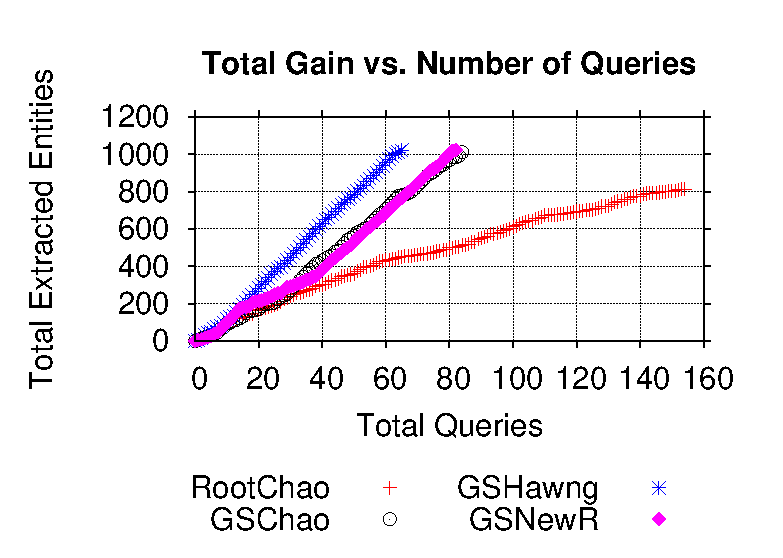
\includegraphics[clip,scale=0.4]{figs/gain_rounds.eps}
	\caption{The number of events extracted by different algorithms for Eventbrite versus the total number of queries.}
	\label{fig:rounds}
	\end{center}
	\vspace{-5pt}
\end{figure}

\noindent{\textbf{How do different CRUX versions traverse the poset and use query configurations?}}
The results reported are averaged over ten runs and correspond to PeopleInNews. We first measure how many queries each algorithm issues at various levels of the poset. In Figure~\ref{fig:level}, we plot the number of queries (per level) issued by our algorithms when the budget is set to 10 and 100 respectively. For a small budget, all algorithms prefer queries at higher levels. The inner nodes are preferred and only a small number of queries is issued at the root (i.e., level one) of the poset. This is justified if we consider that due to their popularity, certain entities are repeatedly extracted, thus, leading to a lower gain. As the budget increases, we see that all algorithms tend to consider more specialized queries at deeper levels of the poset. It is interesting to observe that all algorithms issue the majority of their queries at level two nodes, while GSExact, which has perfect information, focuses mostly on leaf nodes. Thus, our techniques could benefit from being more aggressive at traversing the poset and reaching deeper levels; overall, our techniques may end up being more conservative to cater to a larger space of posets and popularity distributions. In Figure~\ref{fig:queryconf}, we plot the query configurations chosen by our algorithms when the budget is set to 10 and 100. GSExact always prefers queries with $k = 20$ and $l = 0$ for both small and large budgets. On the other hand, our algorithms issue more queries of smaller size when operating under a limited budget and prefer queries of larger size for larger budgets. GSNewR was the only one issuing queries with exclude lists of different sizes, thus, exploiting the rich diversity of query interfaces.


\begin{figure}[h]
    \includegraphics[clip,scale=0.32]{figs/levelBudget10.eps}
	\includegraphics[clip,scale=0.32]{figs/levelBudget100.eps}
	\caption{The number of queries issued at different levels when budget is set at 10 or 100.}\label{fig:level}
\end{figure}

\begin{figure}[h]
   	 \includegraphics[clip,scale=0.32]{figs/queryConfBudget10.eps}
	\includegraphics[clip,scale=0.32]{figs/queryConfBudget100.eps}
	\caption{The query configurations used when budget is set at 10 or 100.}\label{fig:queryconf}
		\vspace{-10pt}
\end{figure}

\noindent{\textbf{Are exclude lists helpful?}} In \Cref{fig:queryconf} we see that only GSNewR made use of exclude lists. However, we observed a drastically different behavior when using a step cost function. \Cref{fig:exEffect} shows the performance of GSChao with and without the use of exclude lists and compares that with the performance of GSExact that uses exclude lists. The results correspond to PeopleInNews. Exploiting exclude lists can yield performance improvements up to 50\% especially for larger budgets.

\begin{figure}[h]
	\begin{center}
	\includegraphics[clip,scale=0.5]{figs/exEffect.eps}
	\caption{Using an exclude list under a step cost function provides significant extraction gains.}
	\label{fig:exEffect}
	\end{center}
	\vspace{-10pt}
\end{figure}

\noindent\textbf{How effective are different estimators at predicting the gain of additional queries?}
GSNewR was able to outperform GSChao and GSHwang for Eventbrite but the opposite behavior was observed for PeopleInNews. To understand the relative performance of the estimators, we measure their error at predicting the number of new retrieved entities for different query configurations for both Eventbrite and PeopleInNews. We summarize our findings. The detailed results are shown in the supplementary material~\cite{cruxsup}.

For large-sparse domains, NewRegr slightly outperforming Chao92Shen and HwangShen for certain queries. For example, for $k = 10, l = 5$, Chao92Shen has a relative error of 0.58, HwangShen had a relative error of 0.7, and NewRegr had a relative error of 0.29. For smaller, dense domains, such as PeopleInNews, NewRegr offers better gain estimates for small query sizes, but as the query size increases, hence, a larger portion of the population is observed, Chao92Shen outperforms both regression-based techniques. 





%!TEX root = ../crux-sigconf.tex


\section{Related Work}
\label{sec:related}
Prior work related to the techniques proposed in this paper can be placed in a few categories; we describe each of them in turn:
\iftr
\vspace{3pt}\noindent\textbf{Crowd Algorithms.} There has been a significant work on designing algorithms where the unit operations 
 (e.g., comparisons, predicate evaluations, and so on) 
 are performed by human workers, including common database primitives such as filter~\cite{crowdscreen}, join~\cite{markus-sorts-joins} and max~\cite{so-who-won},  machine learning primitives, such as entity resolution~\cite{ crowder} and clustering~\cite{crowdclustering}, as well as data mining primitives~\cite{amsterdamer:2013, get-another-label}. 
 \fi
We have already
discussed prior work on crowdsourced extraction or enumeration~\cite{park:2014, trushkowsky:2013} in the introduction. 
\iftr
In both cases, the focus is on a single entity extraction query; extracting entities from large and diverse data domains is not considered. Moreover, the proposed techniques do not support  dynamic querying strategies to optimize for a specified monetary budget. 
\fi

%Finally, to optimize the tradeoff between the gain and cost of queries  previous work proposes either a {\em pay-as-you-go} scheme~\cite{trushkowsky:2013} or a fixed answer size scheme~\cite{park:2014}. In the first case, one repeatedly issues queries to the crowd until the {\em marginal gain}, i.e., the difference between the new extracted entities and the querying cost, drops below a desired threshold. However, the proposed scheme does not enforce any budget constraints explicitly and focuses on a single query in isolation. Thus, it does not optimize the gain-cost tradeoff over an entire querying policy. In the second case, one repeatedly issues queries to the crowd until a desired number of entities is retrieved. The latter is specified by the user. Tthis assumes knowledge of the number of entities to be extracted, which may not be available in many real-world scenarios. 

\vspace{3pt}\noindent\textbf{Knowledge Acquisition Systems.} Recent work has also considered the problem of using crowdsourcing within knowledge acquisition systems~\cite{jiang:13, kondredi:2014, west:2014}. This line of work suggests using the crowd for curating knowledge bases 
\iftr (e.g., assessing the validity of the extracted facts) 
\fi and for gathering additional information to be added to the knowledge base\iftr (e.g., missing attributes of an entity or relationships between entities)\fi, instead of augmenting the set of entities themselves. 
\iftr As a result, these papers are solving an orthogonal problem. The techniques described in this paper for estimating the amount of information from a query and devising querying strategies to maximize the amount of extracted information will surely be beneficial for knowledge extraction systems as well.
\fi

\vspace{3pt}\noindent\textbf{Deep Web Crawling.} A different line of work has focused on data extraction from the deep web~\cite{Jin:2011,Sheng:2012} where data is obtained by querying a form-based interface over a hidden database and extracting results\iftr from dynamically-generated answers (often a list of entities)\fi. Sheng et al.~\cite{Sheng:2012} provide near-optimal algorithms that exploit the exposed structure of the underlying domain to extract all the tuples present in the hidden database. Our goal is similar in that we also extract entities via a collection of interfaces\iftr (in our case the interfaces correspond to queries asked to the crowd)
\fi. Unlike our setting, answers from a hidden database are deterministic, i.e., a query will always retrieve the same top-k tuples. So, it suffices to ask each query precisely once, making it much simpler.
\iftr 
In our setting, since crowdsourced entity extraction queries can be viewed as random samples from an unknown  distribution, one needs to make use of the query result estimation techniques from \Cref{sec:gainestimators}.
\fi
%!TEX root = ../crux.tex

\section{Conclusions and Future Work}
\label{sec:conclusions}
We studied the problem of crowdsourced entity extraction over large and diverse data domains. We proved that the problem of budgeted crowdsourced entity extraction is NP-hard. We introduced CRUX, a novel crowdsourced entity extraction framework, that combines statistical techniques with an adaptive optimization algorithm to maximize the total number of unique entities extracted. We proposed a new regression-based technique for estimating the gain of further querying when the number of retrieved entities is small with respect to the total size of the underlying population. We also introduced a new algorithm that exploits the often known structure of the underlying data domain to devise adaptive querying strategies. CRUX extracts up to 300\% more entities compared to a collection of baselines, and for large sparse entity domains is at most 25\% away from an omniscient adaptive querying strategy with perfect information.

Some of the future directions for extending this work include reasoning about the quality and correctness of the extracted result as well as extending the proposed techniques to other types of information extraction tasks. As mentioned before, the techniques proposed in this paper do not deal with incomplete and imprecise information. However, there has been an increasing amount of literature on addressing these quality issues in crowdsourcing~\cite{ vox-populii, quality, nushi:14, raykar-whom-to-trust}. Combining these techniques, or entity resolution techniques~\cite{crowder} that reason about similarity of extracted entities, with our proposed framework is a promising future direction. Finally, it is of particular interest to apply the proposed framework to other budget sensitive information extraction applications including discovering valuable data sources for integration tasks~\cite{rekatsinas:2015, rekatsinas:2014} or curating an existing knowledge base~\cite{kondredi:2014}.
\balance

%\ifpaper
%\scriptsize
%\fi
{\small 
\bibliographystyle{abbrv}
\bibliography{crux}
}
\end{document}
